\nameref{sub:array}s offer a means of storing and working with a list of values in your code. Each array has a number of elements, each of which has a value, and can be accessed using an index. Together with the \nameref{sub:for_loop}, arrays provide a means of managing multiple values in your code. The following illustrations show how these work in the computer, and should help you better understand how arrays can be used within your code.

\subsection{Understanding \texttt{Populate Array}} % (fold)
\label{sub:understanding_populate_array}

\sref{sub:designing_statistics_calculator} \nameref{sub:designing_statistics_calculator} outlined the pseudocode and flowcharts for a small statistics programs. This included a number of functions and procedures that helped divide the program's code into smaller units of work. One of these procedures was \texttt{Populate Array}, discussed in \sref{ssub:populating_the_array} \nameref{ssub:populating_the_array}. This procedure is responsible for reading values from the user and using these to populate the program's array, and the flowchart for this logic is shown in \fref{fig:populate-array-flow-understanding}.

\begin{figure}[htbp]
   \centering
   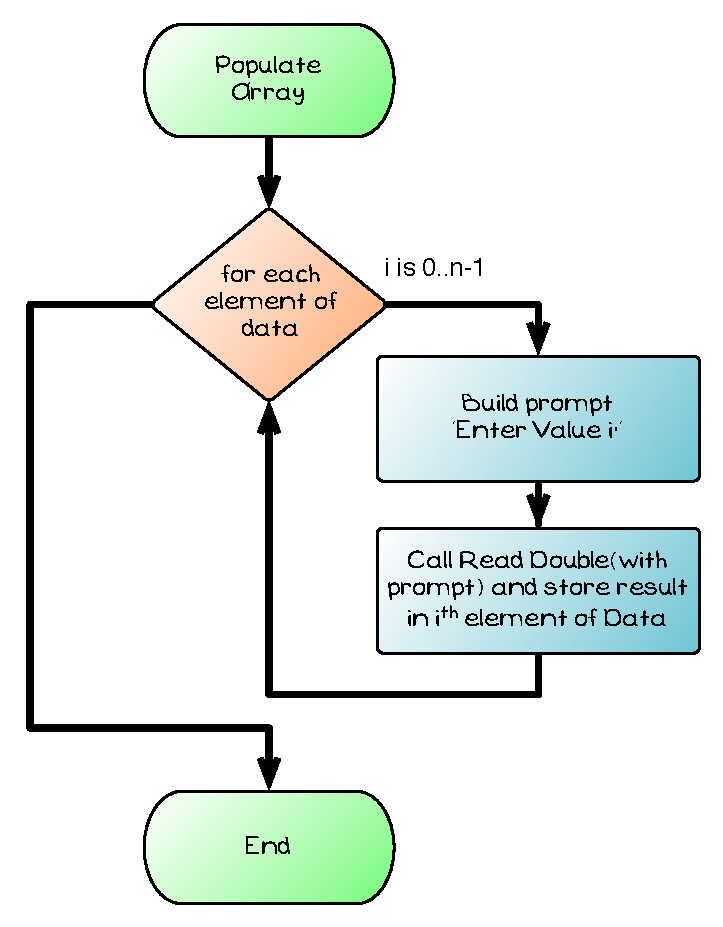
\includegraphics[width=0.5\textwidth]{./topics/arrays/diagrams/PopulateArray} 
   \caption{Flowchart showing the process for \texttt{Populate Array}, from \fref{fig:populate-array-flow}}
   \label{fig:populate-array-flow-understanding}
\end{figure}

The following illustrations will show this code running to populate an array that contains three values. This will show how the array is passed by reference, and how the for loop works together with the array to populate all elements.

\clearpage
\subsubsection{Main starts, and the array is allocated space} % (fold)
\label{ssub:main_starts_and_the_array_is_allocated_space}

All local variables are allocated space on the Stack when the function or procedure they are declared in is called. In this example the \texttt{Main} procedure is executed and space is allocated for its \texttt{my\_data} variable. This variable is an \nameref{sub:array} that is used to store three \texttt{double} values. When \texttt{Main} is loaded onto the Stack there is space allocated for three \texttt{double} values associated with the \texttt{my\_data} variable.

\begin{figure}[htbp]
   \centering
   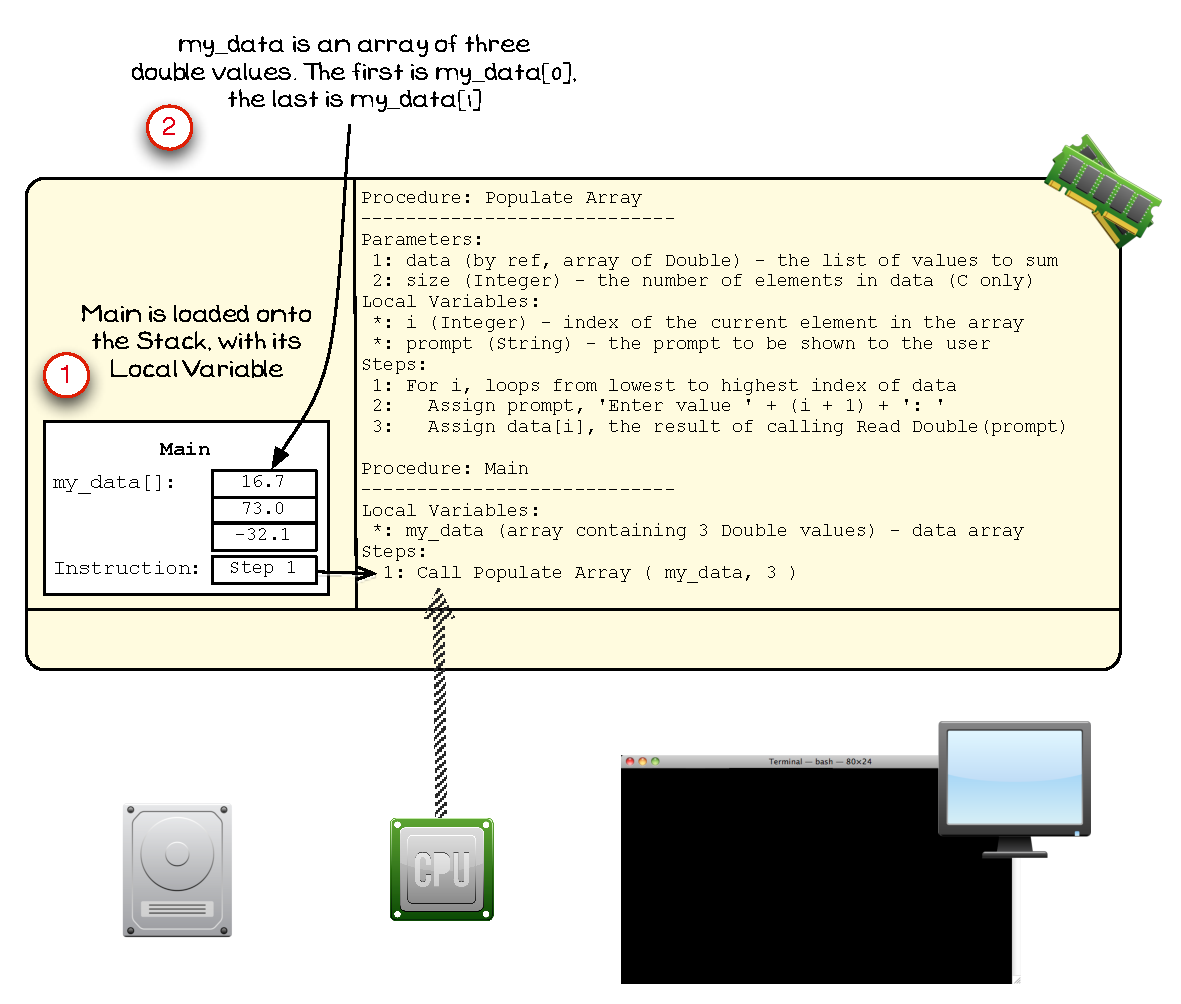
\includegraphics[width=\textwidth]{./topics/arrays/images/PopulateArray1} 
   \caption{When the program starts \texttt{Main} allocates space for its local variables, including the array}
   \label{fig:populate-array-vis-1}
\end{figure}

\mynote{
\begin{itemize}
  \item In \fref{fig:populate-array-vis-1} the indicated areas show the following:
  \begin{enumerate}
    \item The program starts and \texttt{Main} is loaded onto the stack, allocating space for its local variables.
    \item The \texttt{my\_data} array is allocated space to store its values.
  \end{enumerate}
  \medskip
  \item Notice that the three values in the array are allocated next to each other.
  \item The indexes can be used to access the array's elements. The index value determines the number of elements that must be skipped to find where the value is stored.
\end{itemize}
}
% subsubsection main_starts_and_the_array_is_allocated_space (end)

\clearpage
\subsubsection{Populate array is called, and a reference to \texttt{my{\textunderscore}data} passed in} % (fold)
\label{ssub:populate_array_is_called_and_a_reference_to_my_data_passed_in}

\texttt{Populate Array} is called as the first step in \texttt{Main}. This is passed the \texttt{my\_data} variable (pass by reference), rather than being passed the values from within that variable. This gives the \texttt{data} parameter access to the memory where \texttt{my\_data} is stored.

\begin{figure}[htbp]
   \centering
   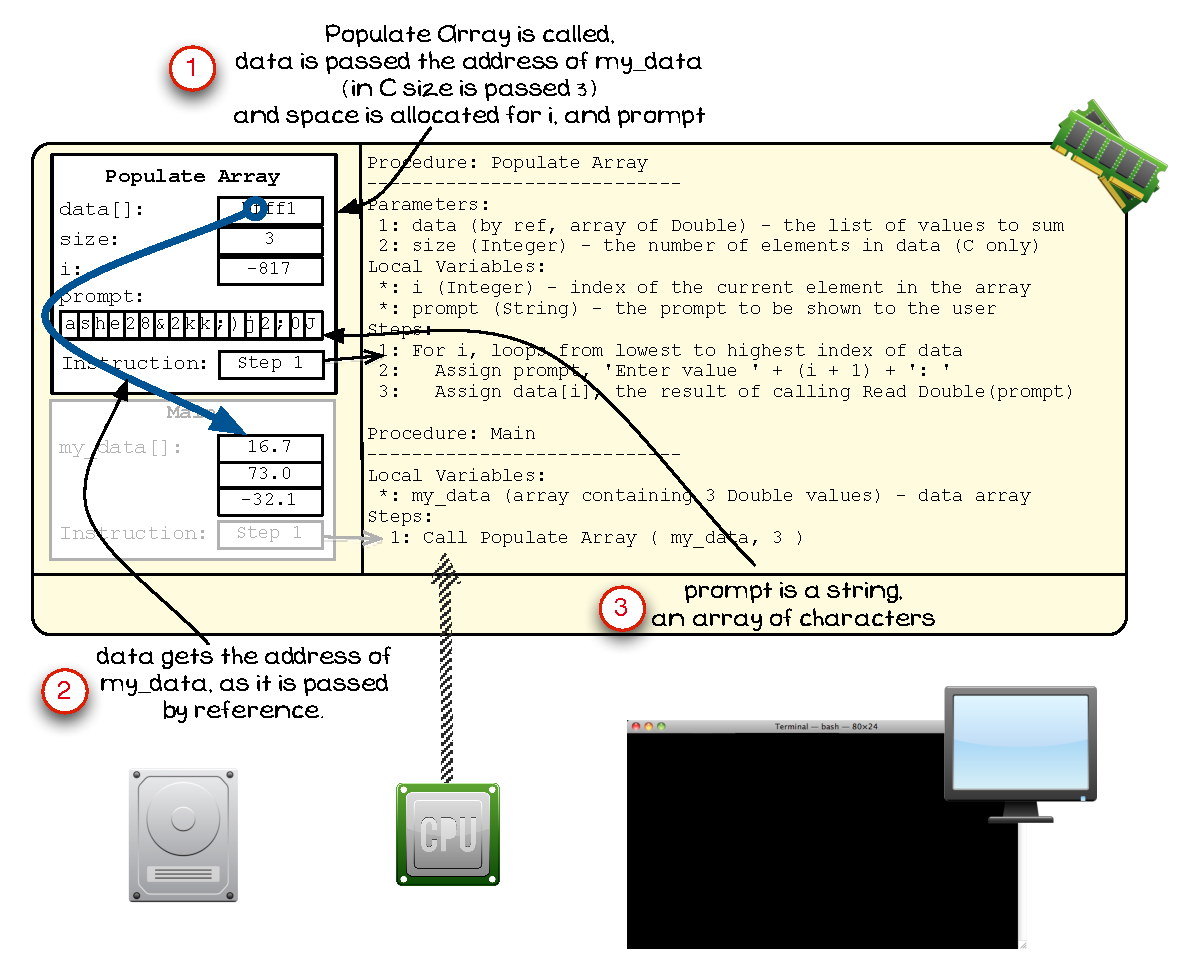
\includegraphics[width=\textwidth]{./topics/arrays/images/PopulateArray2} 
   \caption{Populate array is called, and a reference to the \texttt{my\_data} array is pass to its \texttt{data} parameter}
   \label{fig:populate-array-vis-2}
\end{figure}

\mynote{
\begin{itemize}
  \item In \fref{fig:populate-array-vis-2} the indicated areas show the following:
  \begin{enumerate}
    \item When \texttt{Populate Array} is called it is loaded onto the Stack. Its \texttt{data} parameter receives the address of \texttt{my\_data} from \texttt{Main}. In C the value 3 would also be passed to the \texttt{size} parameter, as C does not keep track of the length of the array for you. At the same time space for \texttt{Populate Array}'s local variables \texttt{i} and \texttt{prompt} are allocated on the Stack.
    \item Notice that in \texttt{Populate Array} the \texttt{data} parameter only stores the address of the array, as it is passed by reference. This saves time and space, and is needed in this case as the procedure wants to store data into the variable passed to this parameter.
    \item The \texttt{prompt} local variable is also an array. It is allocated spaces on the stack as is done for all local variables. 
  \end{enumerate}
  \medskip
  \item Arrays are allocated a contiguous area of memory to store its elements.
  \item A String is an array of characters.
\end{itemize}
}

% subsubsection populate_array_is_called_and_a_reference_to_my\_data_passed_in (end)

\clearpage
\subsubsection{Step 1 of \texttt{Populate Array} is run} % (fold)
\label{ssub:step_1_of_populate_array_is_run}

Step 1 of \texttt{Populate Array} initialises the for loop's control variable (\texttt{i} in this case). This variable keeps track of the times the loop body has executed, and can be used to get the \emph{current} value from the array.

\begin{figure}[htbp]
   \centering
   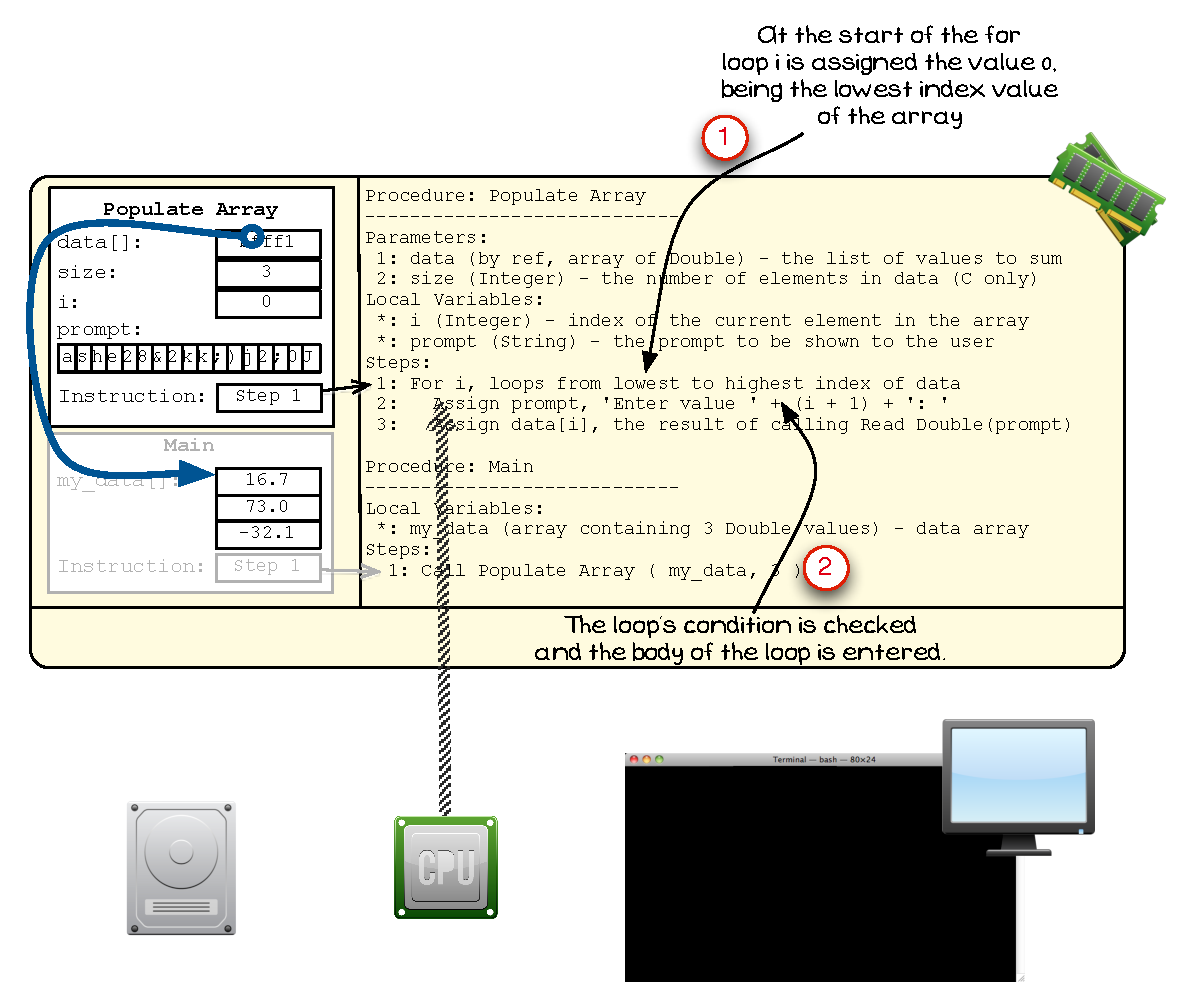
\includegraphics[width=\textwidth]{./topics/arrays/images/PopulateArray3} 
   \caption{Step 1 of \texttt{Populate Array} is called, and the for loop sets i to the lowest index of the \texttt{data} array}
   \label{fig:populate-array-vis-3}
\end{figure}

\mynote{
\begin{itemize}
  \item In \fref{fig:populate-array-vis-3} the indicated areas show the following:
  \begin{enumerate}
    \item Step 1 of \texttt{Populate Array} is a for loop. The first action of the for loop is to initialise the value of \texttt{i} to the \emph{lowest index value} of the \texttt{data} array. The lowest index is 0, so \texttt{i} is assigned the value 0.
    \item Next the loop checks its condition, it is loop from 0 to 2, and has not passed 2 so the body of the loop will be executed. This will be checked again when the for loop ends.
  \end{enumerate}
  \medskip
  \item The first action of a for loop is to initialise the value of the control variable.
  \item When processing each element of an array the for loop should initialise the control variable to 0, the first index of the array.
\end{itemize}
}

% subsubsection step_1_of_populate_array_is_run (end)

\clearpage
\subsubsection{Step 2 constructs the prompt to be shown to the user} % (fold)
\label{ssub:step_2_constructs_the_prompt_to_be_shown_to_the_user}

The user needs to be told what to enter. The \texttt{prompt} is a string that will contain this message so that it can be passed to \texttt{Read Double}. The value for the prompt will use the loop's control variable (the counter) so that the user known which value they are up to.

\begin{figure}[htbp]
   \centering
   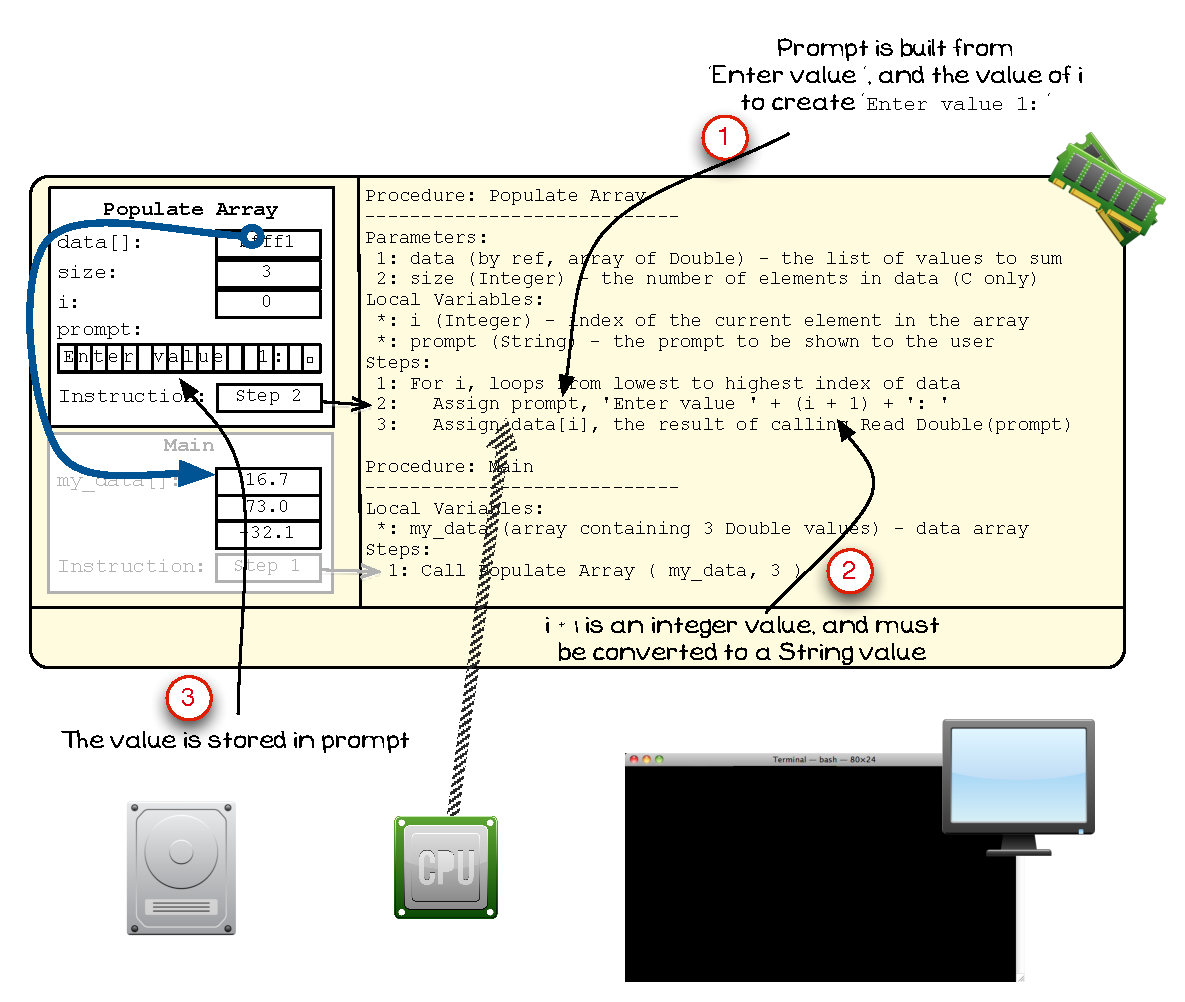
\includegraphics[width=\textwidth]{./topics/arrays/images/PopulateArray4} 
   \caption{Step 2 builds the prompt \texttt{Enter value 1: } which will be shown to the user}
   \label{fig:populate-array-vis-4}
\end{figure}

\mynote{
\begin{itemize}
  \item In \fref{fig:populate-array-vis-4} the indicated areas show the following:
  \begin{enumerate}
    \item Step 2 of \texttt{Populate Array} builds the prompt by concatenating `\texttt{Enter Value}' with \texttt{i + 1} and `\texttt{: }'.
    \item To achieve this \texttt{i + 1} must be converted from an Integer to a String.
    \item The result is stored in the \texttt{prompt} variable.
  \end{enumerate}
  \medskip
  \item This action will be performed each time the loop executes. In this case the value stored in \texttt{prompt} will be `\texttt{Enter value  1: }'.
  \item The small square shown at the end of the \texttt{prompt} represents the overhead. In C this is the \emph{sentinel} value, in Pascal it is the length\footnote{Pascal actually stores the length at the start of the string, but the idea is the same.} of the array.
\end{itemize}
}


% subsubsection step_2_constructs_the_prompt_to_be_shown_to_the_user (end)

\clearpage
\subsubsection{Step 3 reads a value from the user and stores it in the array at index 0} % (fold)
\label{ssub:step_3_reads_a_value_from_the_user_and_stores_it_in_the_array_at_index_0}

The next step calls the \texttt{Read Double} function. This is responsible for reading a value from the user, and returning it to the caller. The value returned is then stored in an element of the array. The \texttt{i} variable is read to determine the position where this value should be stored. This means that you can think of \texttt{i} as referring to the \emph{current} element of the array.

\begin{figure}[htbp]
   \centering
   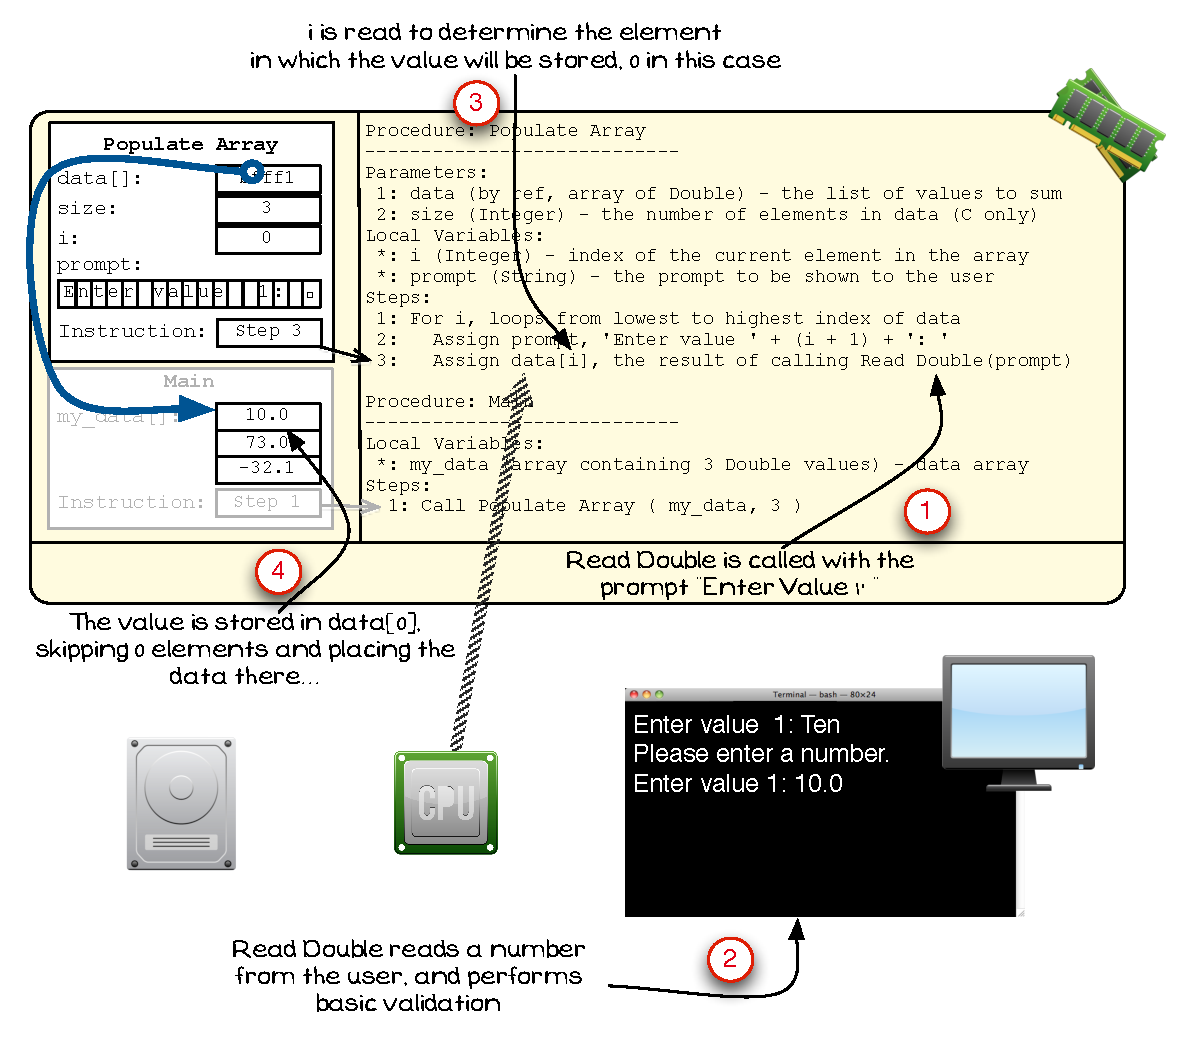
\includegraphics[width=\textwidth]{./topics/arrays/images/PopulateArray5} 
   \caption{Step 3 reads a \texttt{double} value from the user and stores it in \texttt{data[i]}}
   \label{fig:populate-array-vis-5}
\end{figure}

\mynote{
\begin{itemize}
  \item In \fref{fig:populate-array-vis-5} the indicated areas show the following:
  \begin{enumerate}
    \item Step 3 of \texttt{Populate Array} calls \texttt{Read Double}, passing across the prompt to be shown to the user.
    \item Within \texttt{Read Double} the value is read from the Terminal. This includes some validation to make sure that the value entered is a number.
    \item To determine where the value is stored the computer needs to evaluate the expression used to index the array. In this case that is the value of the \texttt{i} variable.
    \item The \texttt{data} reference is followed, and \texttt{0} elements skipped, to find the location where the data should be stored. 
  \end{enumerate}
  \medskip
  \item Notice that this has stored the value in \texttt{my\_data}, as \texttt{data} is passed by reference.
\end{itemize}
}

% subsubsection step_3_reads_a_value_from_the_user_and_stores_it_in_the_array_at_index_0 (end)

\clearpage
\subsubsection{Control returns to Step 1 as the loop body has ended} % (fold)
\label{ssub:control_returns_to_step_1_as_the_loop_body_has_ended}

At the end of the loop body the for loop performs two actions. It has finished the first pass through the loop, so its control variable (the counter) needs to be incremented to 1. Then it needs to jump back to check its condition. This will determine if the loop's body is executed again or skipped. In this case \texttt{i} is still in the defined range so the loop's body is run again.

\begin{figure}[htbp]
   \centering
   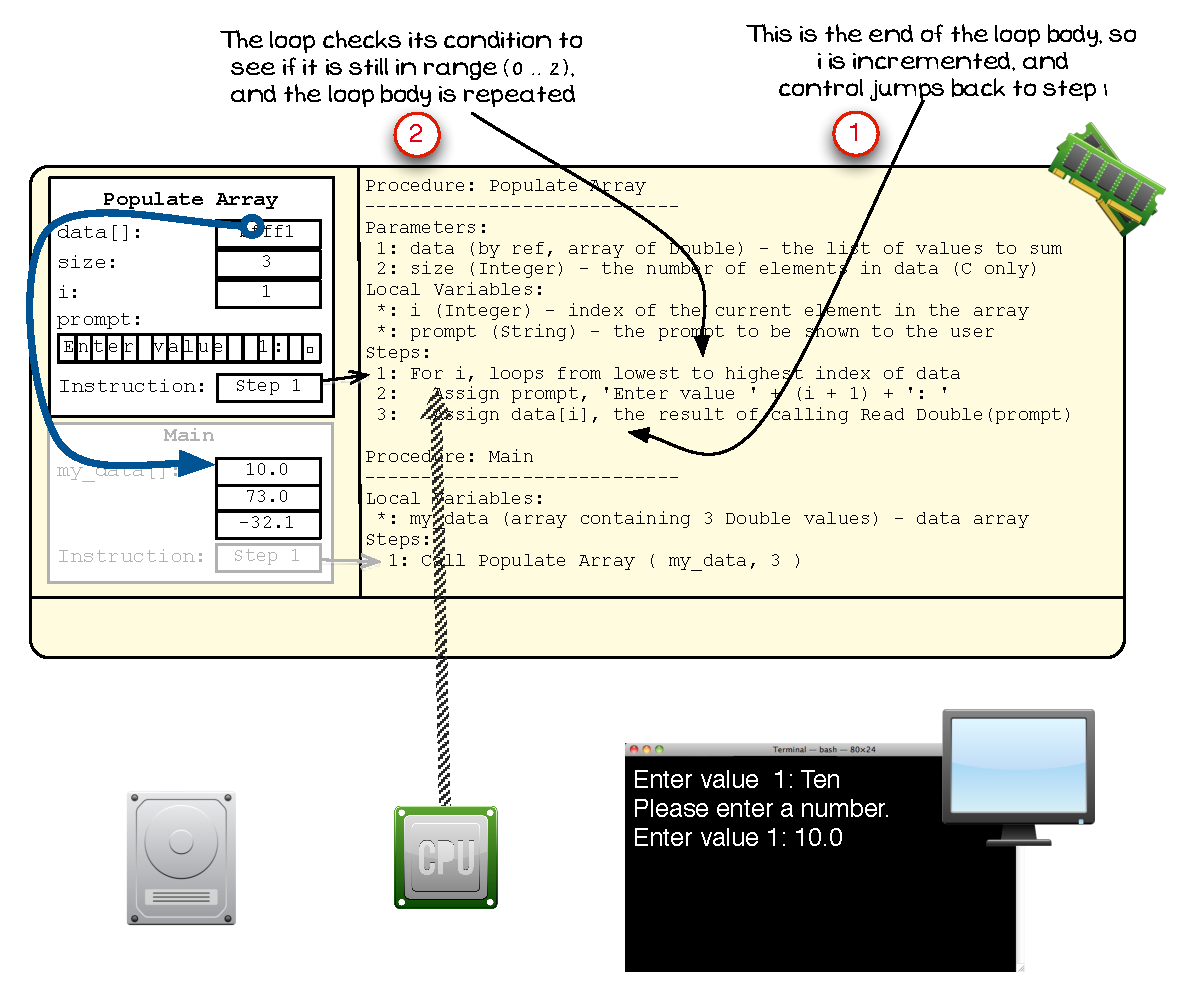
\includegraphics[width=\textwidth]{./topics/arrays/images/PopulateArray6} 
   \caption{At the end of the loop body \emph{i} is incremented and control jumps back to check the loop's condition}
   \label{fig:populate-array-vis-6}
\end{figure}

\mynote{
\begin{itemize}
  \item In \fref{fig:populate-array-vis-6} the indicated areas show the following:
  \begin{enumerate}
    \item The end of the loop body indicates that two things needs to occur. Firstly the value of \texttt{i} needs to be incremented, and then control needs to jump back to check the condition of the loop (step 1).
    \item The loop's condition checks if \texttt{i} is still in range (\texttt{i} is in the range \texttt{0..2}, coded as \texttt{i < size} in C). As it is still in range the loop's body will execute again.
  \end{enumerate}
  \medskip
\end{itemize}
}

% subsubsection control_returns_to_step_1_as_the_loop_body_has_ended (end)

\clearpage
\subsubsection{Second prompt is built asking the user to enter value 2} % (fold)
\label{ssub:second_prompt_is_built_asking_the_user_to_enter_value_2}

Back at step 2 again, the prompt needs to be recreated. This time its message will be `\texttt{Enter value 2: }'. The process to create this is the same, with the value of \texttt{i + 1} being converted to a String, and the three parts concatenated together and stored in \texttt{prompt}. This overrides the details in the existing array, reusing the same memory to store these values.

\begin{figure}[htbp]
   \centering
   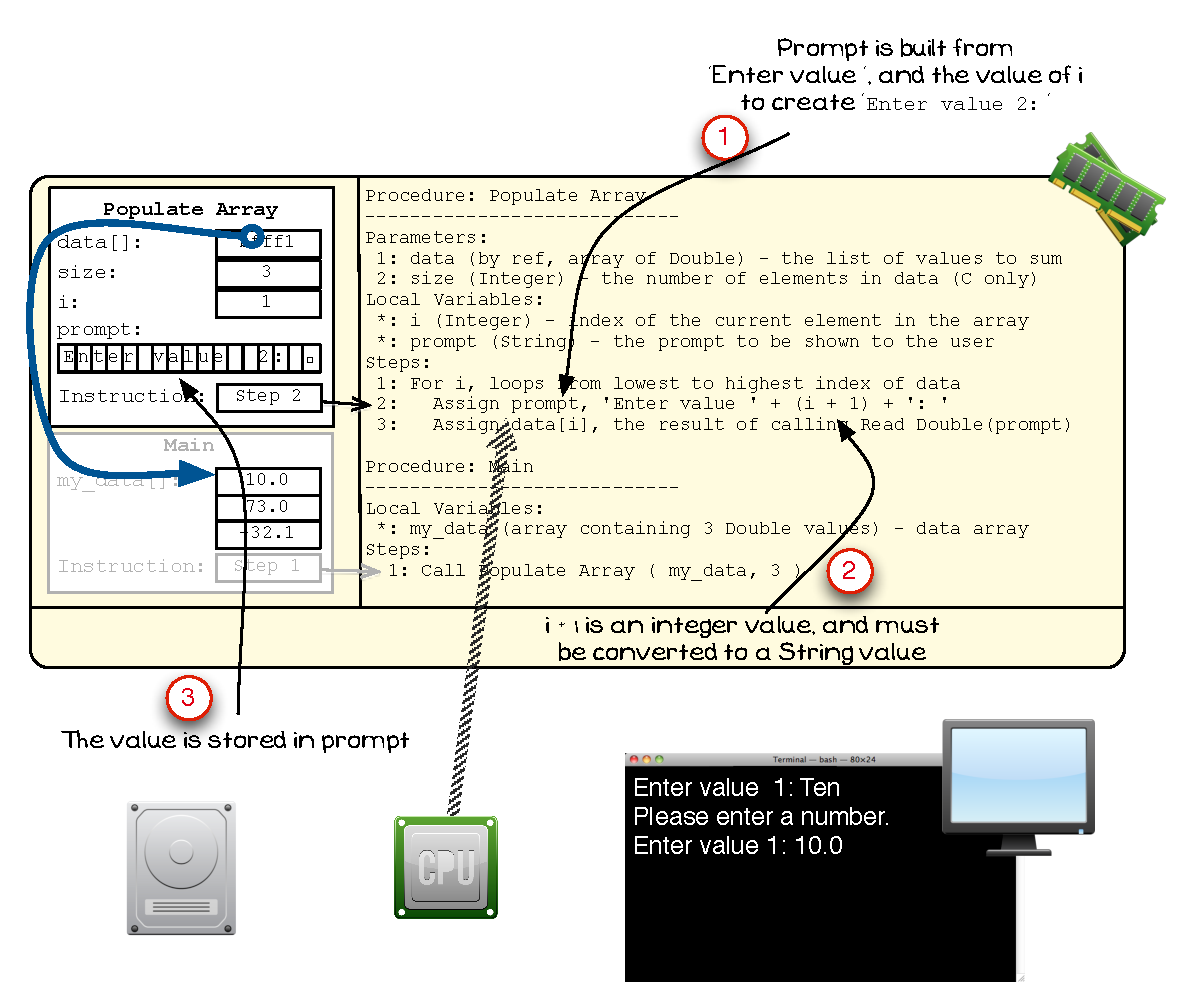
\includegraphics[width=\textwidth]{./topics/arrays/images/PopulateArray7} 
   \caption{Step 2 builds the prompt \texttt{Enter value 2: } which will be shown to the user}
   \label{fig:populate-array-vis-7}
\end{figure}

\mynote{
\begin{itemize}
  \item In \fref{fig:populate-array-vis-7} the indicated areas show the following:
  \begin{enumerate}
    \item Step 2 of \texttt{Populate Array} builds the prompt by concatenating `\texttt{Enter Value}' with \texttt{i + 1} and `\texttt{: }'.
    \item To achieve this \texttt{i + 1} must be converted from an Integer to a String.
    \item The result is stored in the \texttt{prompt} variable.
  \end{enumerate}
  \medskip
  \item Notice that this is using the same location to store its data.
  \item The small square shown at the end of the \texttt{prompt} represents the overhead. In C this is the \emph{sentinel} value, in Pascal it is the length\footnote{Pascal actually stores the length at the start of the string, but the idea is the same.} of the array.
\end{itemize}
}

% subsubsection second_prompt_is_built_asking_the_user_to_enter_value_2 (end)

\clearpage
\subsubsection{\texttt{Populate Array} stores the second value read into \texttt{data[1]}} % (fold)
\label{ssub:populate_array_stores_the_second_value_read_into_data[1]}

Step 3 uses \texttt{Read Double} again to get the value to store in the second element of the array. To find where this should be stored the computer calculates the value of the index, reading this from the \texttt{i} variable. The value returned from \texttt{Read Double} is then stored in the array referred to by \texttt{data}, at index \texttt{1}.

\begin{figure}[htbp]
   \centering
   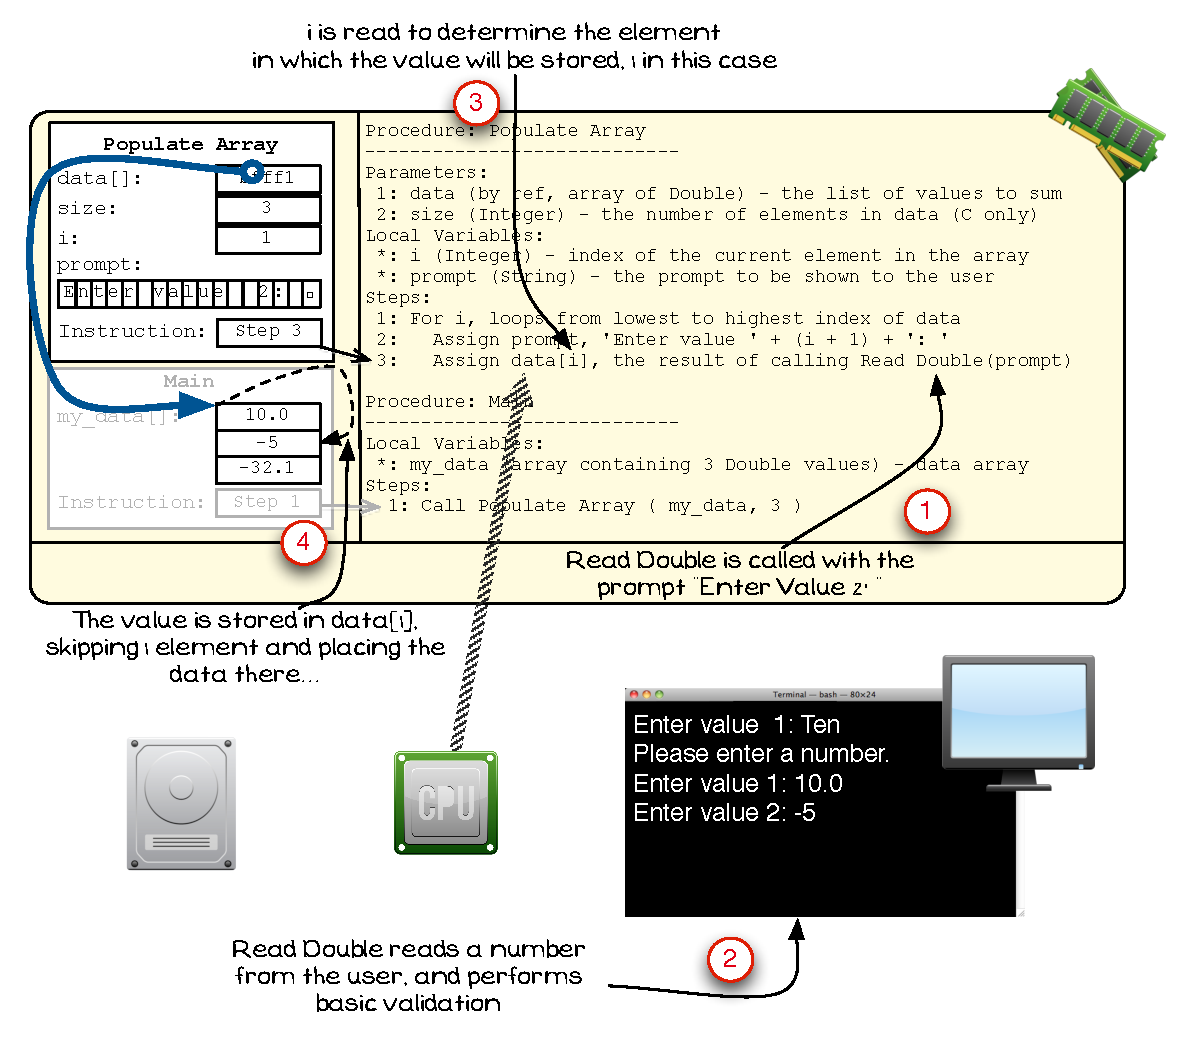
\includegraphics[width=\textwidth]{./topics/arrays/images/PopulateArray8} 
   \caption{The second value read is stored in \texttt{data[1]}}
   \label{fig:populate-array-vis-8}
\end{figure}

\mynote{
\begin{itemize}
  \item In \fref{fig:populate-array-vis-8} the indicated areas show the following:
  \begin{enumerate}
    \item Step 3 of \texttt{Populate Array} calls \texttt{Read Double}, passing across the prompt to be shown to the user.
    \item Within \texttt{Read Double} the value is read from the Terminal. This includes some validation to make sure that the value entered is a number.
    \item The value of the index is now \texttt{1}, as read from variable \texttt{i}.
    \item The \texttt{data} reference is followed, and \texttt{1} element is skipped, to find the location where the data should be stored.
  \end{enumerate}
  \medskip
\end{itemize}
}

% subsubsection populate_array_stores_the_second_value_read_into_data[1] (end)

\clearpage
\subsubsection{\texttt{i} is incremented again, and control returns to Step 1 to determine if loop runs again} % (fold)
\label{ssub:i_is_incremented_again_and_control_returns_to_step_1_to_determine_if_loop_runs_again}

The end of the for loop's body has been reached again, so it performs two actions: it increments its control variable (\texttt{i} in this case) and jumps back to check its condition (step 1). The condition then determines if the loop's body is to be executed again or skipped. In this case \texttt{i} is still in the defined range so the loop's body is run a third time.

\begin{figure}[htbp]
   \centering
   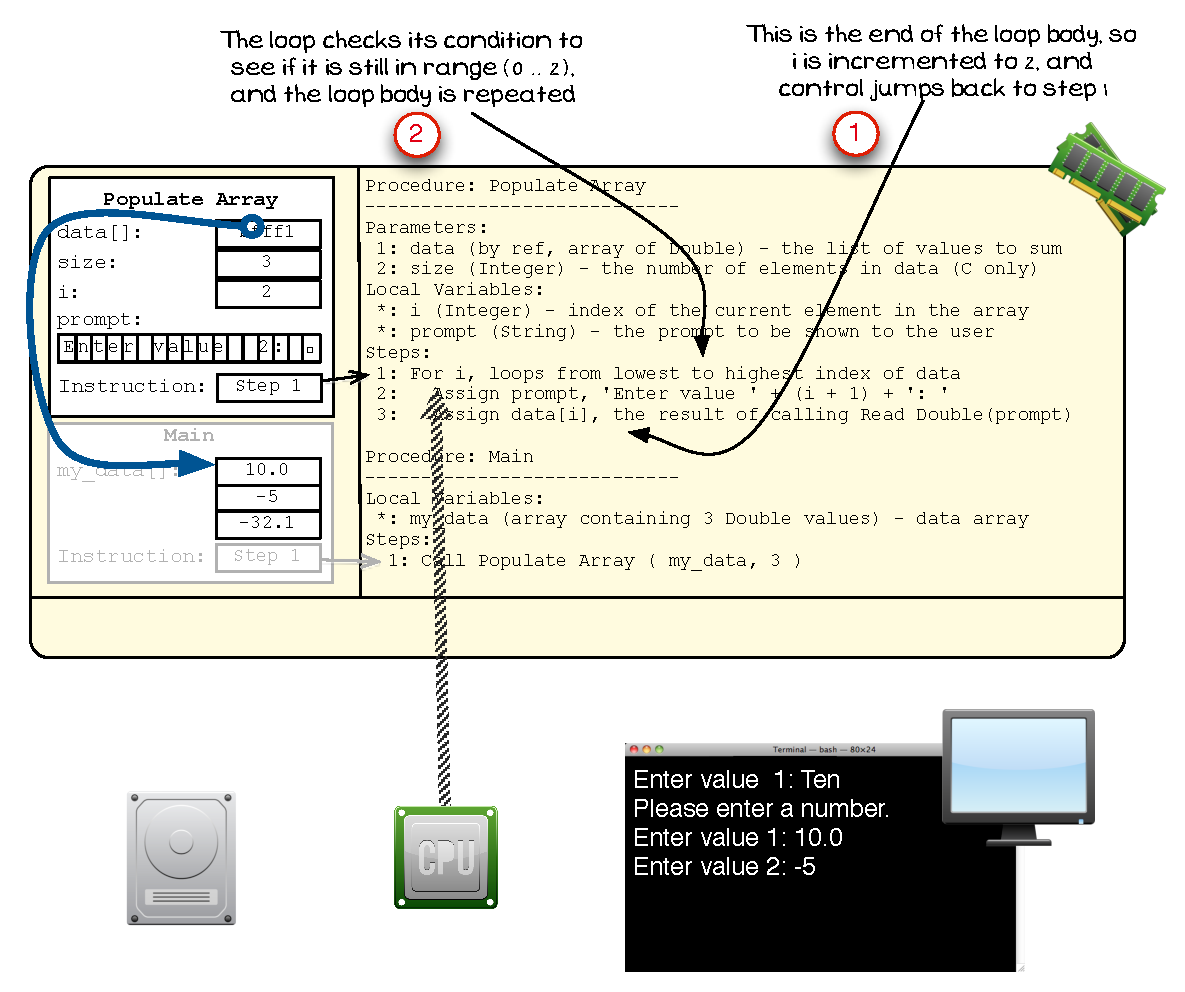
\includegraphics[width=0.98\textwidth]{./topics/arrays/images/PopulateArray9} 
   \caption{At the end of the loop body \emph{i} is incremented and control jumps back to check the loop's condition}
   \label{fig:populate-array-vis-9}
\end{figure}

\mynote{
\begin{itemize}
  \item In \fref{fig:populate-array-vis-9} the indicated areas show the following:
  \begin{enumerate}
    \item The end of the loop body indicates that two things needs to occur: the value of \texttt{i} is incremented, and control jump back to check the condition of the loop.
    \item The loop's condition checks if \texttt{i} is still in range (\texttt{i} is in the range \texttt{0..2}, coded as \texttt{i < size} in C). As it is still in range the loop's body is execute again.
  \end{enumerate}
  \medskip
  \item These same actions always occur at the end of the for loop. It increments its control variable, and jumps back to check its condition.
\end{itemize}
}

\csection{The C for loop can be used for more than just counting. At the end of the loop the instructions from the \nameref{sub:c_for_loop}'s \emph{increment} occur, typically something like \texttt{i++}.}


% subsubsection i_is_incremented_again_and_control_returns_to_step_1_to_determine_if_loop_runs_again (end)

\clearpage
\subsubsection{Third prompt is built asking the user to enter value 3} % (fold)
\label{ssub:third_prompt_is_built_asking_the_user_to_enter_value_3}

Back at step 2 for the third time. This step recreates the prompt, this time with the message `\texttt{Enter value 3: }'. The process to create this is the same as before, with the value of \texttt{i + 1} being converted to a String, and the three parts concatenated together and stored in \texttt{prompt}. Remember that this overrides the data currently in the \texttt{prompt} array.

\begin{figure}[htbp]
   \centering
   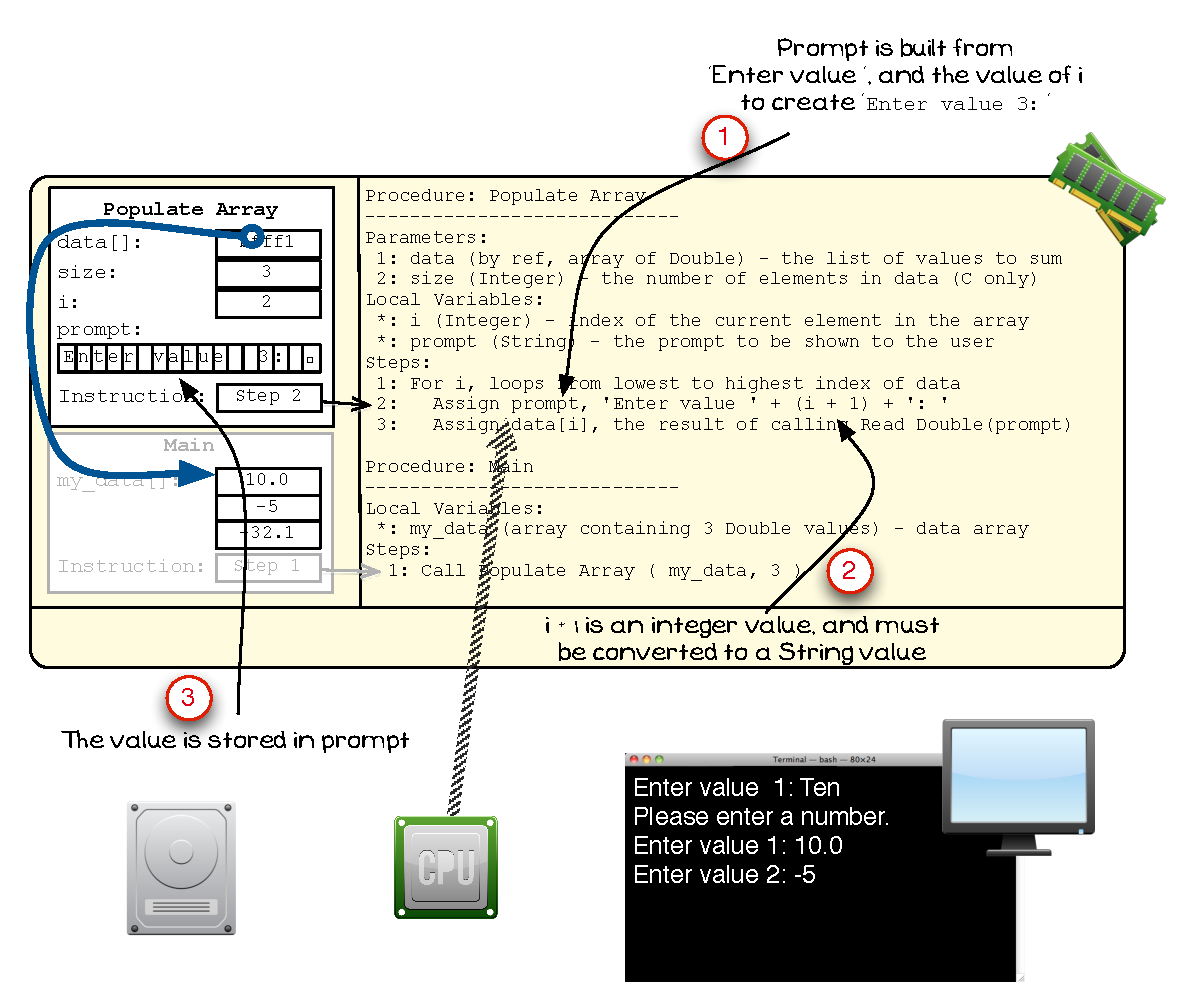
\includegraphics[width=\textwidth]{./topics/arrays/images/PopulateArray10} 
   \caption{Step 2 builds the prompt \texttt{Enter value 3: } which will be shown to the user}
   \label{fig:populate-array-vis-10}
\end{figure}

\mynote{
\begin{itemize}
  \item In \fref{fig:populate-array-vis-10} the indicated areas show the following:
  \begin{enumerate}
    \item Step 2 of \texttt{Populate Array} builds the prompt by concatenating `\texttt{Enter Value}' with \texttt{i + 1} and `\texttt{: }'.
    \item To achieve this \texttt{i + 1} must be converted from an Integer to a String.
    \item The result is stored in the \texttt{prompt} variable.
  \end{enumerate}
  \medskip
\end{itemize}
}

% subsubsection third_prompt_is_built_asking_the_user_to_enter_value_3 (end)

\clearpage
\subsubsection{\texttt{Populate Array} stores the third value read into \texttt{data[2]}} % (fold)
\label{ssub:populate_array_stores_the_third_value_read_into_data[2]}

Once again, step 3 uses \texttt{Read Double} get the value to store in the array. In this case \texttt{i} indicates that this should be stored in the element at index 2 (skipping 2 elements, so storing the value in the third).

\begin{figure}[htbp]
   \centering
   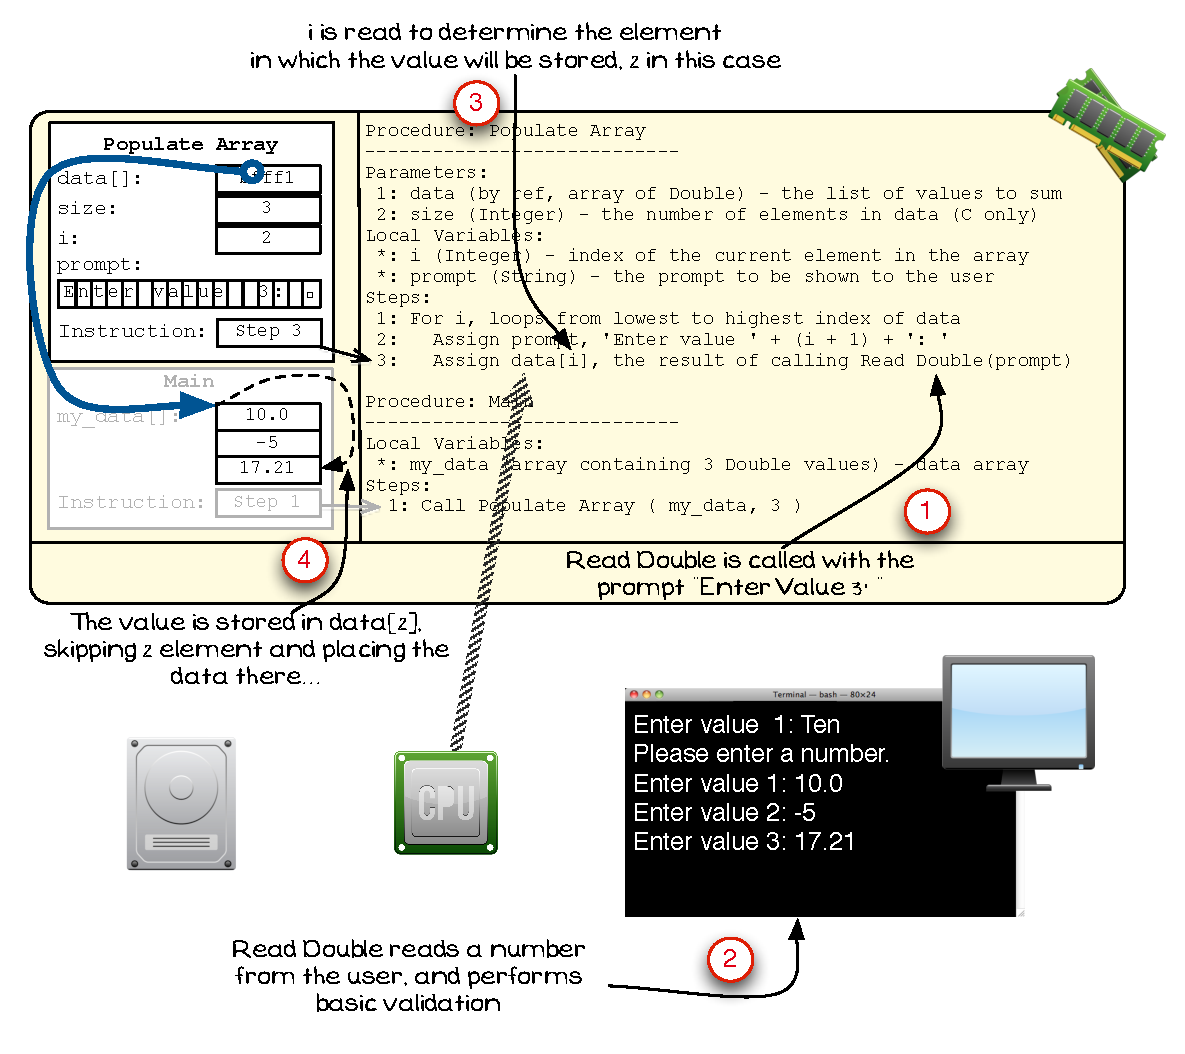
\includegraphics[width=\textwidth]{./topics/arrays/images/PopulateArray11} 
   \caption{The second value read is stored in \texttt{data[1]}}
   \label{fig:populate-array-vis-11}
\end{figure}

\mynote{
\begin{itemize}
  \item In \fref{fig:populate-array-vis-11} the indicated areas show the following:
  \begin{enumerate}
    \item Step 3 of \texttt{Populate Array} calls \texttt{Read Double} again.
    \item Within \texttt{Read Double} the value is read from the Terminal.
    \item The value of the index is now \texttt{2}, as read from variable \texttt{i}.
    \item The \texttt{data} reference is followed, and \texttt{2} elements are skipped to find the location where the data should be stored.
  \end{enumerate}
  \medskip
  \item Notice how over these three loops \texttt{i} has been used to determine which element is the \emph{current element}. The loop's processing is the same, but changing \texttt{i} means that this action is applied to each element in the array one at a time.
  \item The loop's body determines the action to apply to the \texttt{$i^{th}$} element of the array.
  \item The for loop then updates \texttt{i} so that the body is applied to \emph{each} element of the array.
\end{itemize}
}

% subsubsection populate_array_stores_the_third_value_read_into_data[2] (end)

\clearpage
\subsubsection{\texttt{i} is incremented again, and control jumps back to check the condition a fourth time} % (fold)
\label{ssub:i_is_incremented_again_and_control_jumps_back_to_check_the_condition_a_fourth_time}

The end of the for loop's body has been reached again, so it performs two actions: it increments its control variable (\texttt{i} in this case) and jumps back to check its condition (step 1). This time the value of \texttt{i} is outside the range of the indexes for \texttt{data} (\texttt{0..2}, it is no longer less than 3). This means that the loop's body should not be run again, and control will jump past the body to the next step. As there are no more steps in \texttt{Populate Array} it will end.

\begin{figure}[htbp]
   \centering
   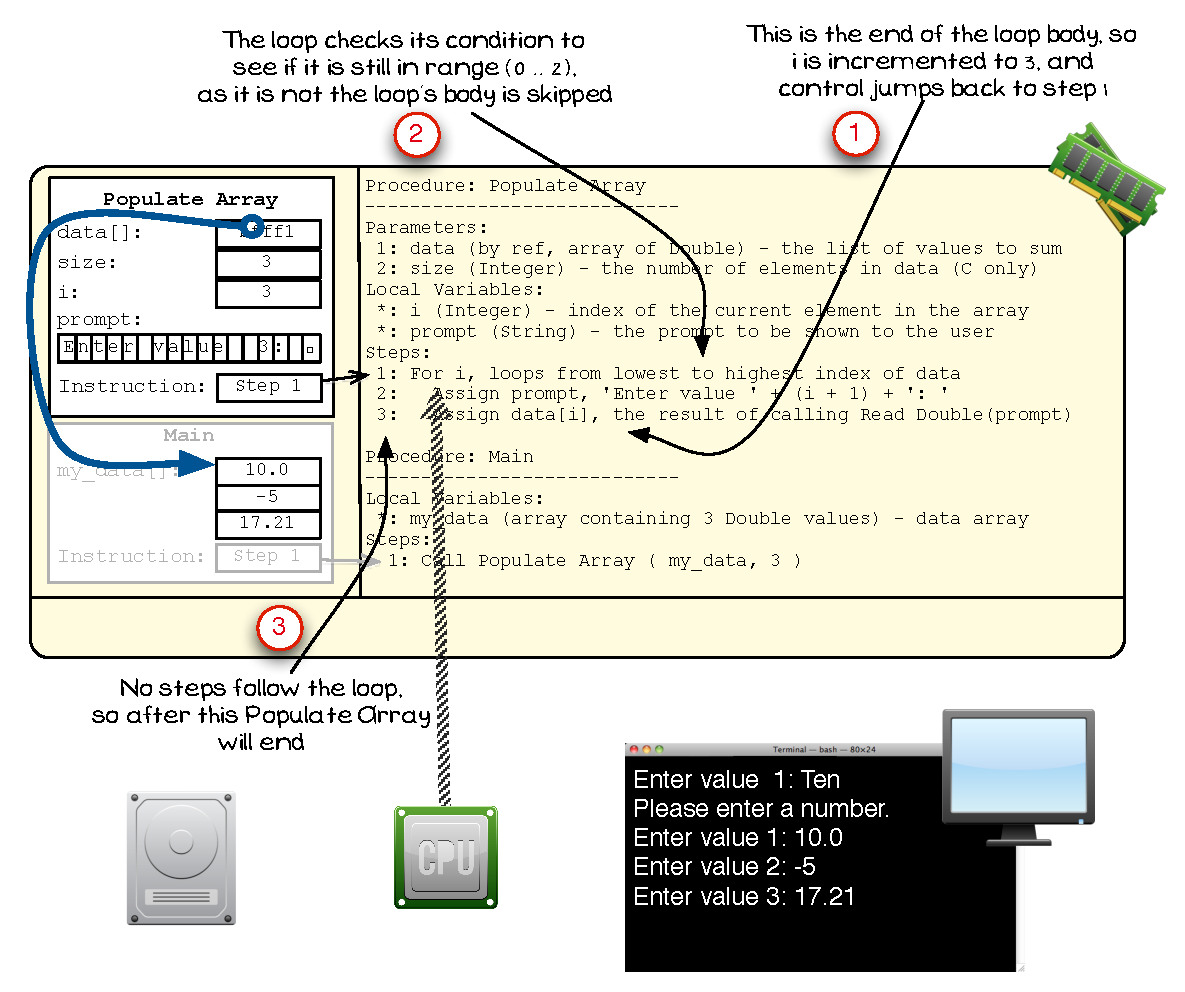
\includegraphics[width=\textwidth]{./topics/arrays/images/PopulateArray12} 
   \caption{At the end of the loop body \emph{i} is incremented and control jumps back to check the loop's condition}
   \label{fig:populate-array-vis-12}
\end{figure}

\mynote{
\begin{itemize}
  \item In \fref{fig:populate-array-vis-12} the indicated areas show the following:
  \begin{enumerate}
    \item The end of the loop body causes the value of \texttt{i} to be incremented, and control jump back to check the condition of the loop.
    \item The loop's condition checks if \texttt{i} is still in range (\texttt{i} is in the range \texttt{0..2}, coded as \texttt{i < size} in C).
    \item \texttt{i} is \textbf{not} in the range \texttt{0..2}, so the loop body is skipped. As there are no more steps in this procedure it ends.
  \end{enumerate}
  \medskip
  \item The condition in the for loop is responsible for determining if the loop runs again. This time the condition indicates that the loop is not to be run again, so control will jump past the end of the loop.
  \item The for loop works like a while loop, with additional logic to keep a counter.
\end{itemize}
}

% subsubsection i_is_incremented_again_and_control_jumps_back_to_check_the_condition_a_fourth_time (end)

\clearpage
\subsubsection{\texttt{Populate Array} ends, and has populated \texttt{Main}'s \texttt{my{\textunderscore}data} array} % (fold)
\label{ssub:populate_array_ends_and_has_populated_main_s_my_data_array}

When \texttt{Populate Array} ends its space on the stack is released so that it can be used again, and control returns to \texttt{Main}. \texttt{Populate Array} was responsible for reading values from the user and storing these in the array passed to it, and if you look at \fref{fig:populate-array-vis-13} you can see that this has been achieved.

The instructions in \texttt{Populate Array} commanded the computer to read a value from the user and store it in the current element (the $i^{th}$ element) of the array. These actions were then repeated by the \nameref{sub:for_loop} \emph{for each} index of the array. Together the for loop and its body allow you to define actions that must be performed on all elements in an array.

\begin{figure}[htbp]
   \centering
   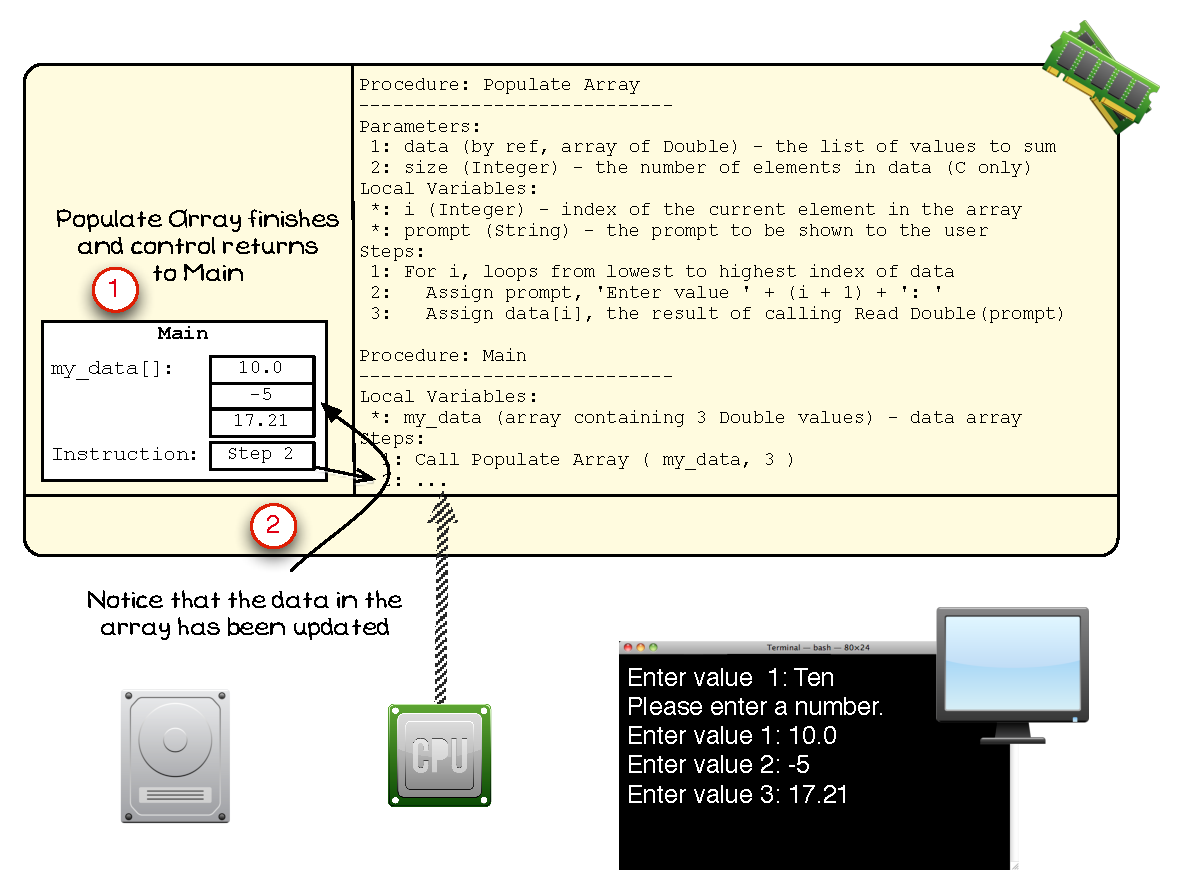
\includegraphics[width=\textwidth]{./topics/arrays/images/PopulateArray13} 
   \caption{Control returns to \texttt{Main}, and its \texttt{my\_data} array has been populated}
   \label{fig:populate-array-vis-13}
\end{figure}

\mynote{
\begin{itemize}
  \item In \fref{fig:populate-array-vis-13} the indicated areas show the following:
  \begin{enumerate}
    \item The last step in \texttt{Populate Array} has been completed, so it ends and control returns to \texttt{Main}.
    \item The values in \texttt{my\_data} have been updated. Passing this array by reference to \texttt{Populate Array} allowed it to make changes to this array's values.
  \end{enumerate}
  \medskip
  \item Notice that the data associated with the \texttt{Populate Array} procedure has been released, including the data used for the \texttt{prompt} array.
  \item \texttt{Populate Array} is responsible for filling the array passed to it with values from the user, and that is what it has done.
  
\end{itemize}
}

% subsubsection populate_array_ends_and_has_populated_main_s_my_data_array (end)
% subsection understanding_populate_array (end) 

\clearpage
\subsection{Understanding \texttt{Sum}} % (fold)
\label{sub:understanding_sum}

\fref{fig:sum-understanding} shows the flowchart of the \texttt{Sum} function from the Statistics Calculator program. This algorithm was developed in the \sref{ssub:calculating_sum}, and its Pseudocode is shown in Listing \ref{plst:sum}. The \texttt{Sum} function is responsible for calculating the sum of all of the values in the array passed to it. This is achieved by having a \texttt{total} variable that is initialised to 0, and then has the value of \emph{each element} from the array added to it.

\begin{figure}[htbp]
   \centering
   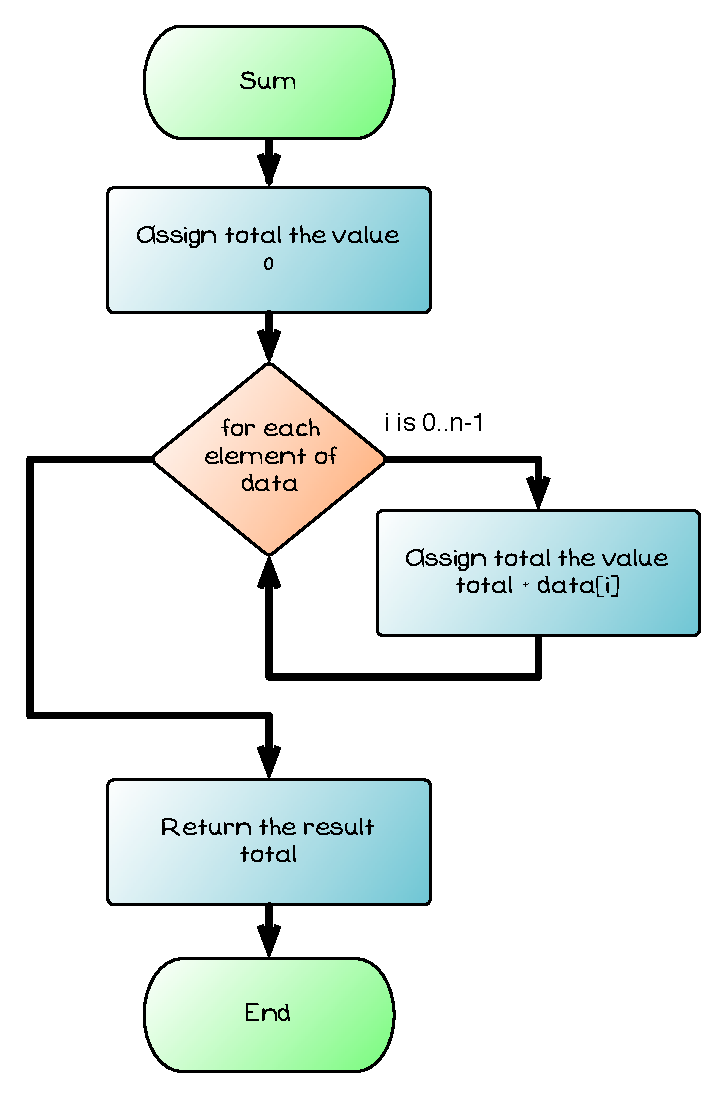
\includegraphics[width=0.5\textwidth]{./topics/arrays/diagrams/SumFlow} 
   \caption{Flowchart showing the process for \texttt{Sum}}
   \label{fig:sum-understanding}
\end{figure}

The following code will show how this function is executed on an array with three values in it. This will continue the execution from \sref{sub:understanding_populate_array} \nameref{sub:understanding_populate_array}, though the same process would occur for any array values.

\mynote{
The most important thing to pay attention to in this illustration is the interactions between the \nameref{sub:for_loop} and the \nameref{sub:array}. Make sure you can see how this combination allows you to specify the actions to be performed on an element (in the loop's body), and then to have this run for each element of the array (controlled by the loop condition).
}

\clearpage
\subsubsection{\texttt{Sum} is called, and passed the \texttt{my data} array} % (fold)
\label{ssub:sum_is_called_and_passed_the_values_in_my_data}

When \texttt{Sum} is called it is passed the array to read its values from. This is passed in the same way as was done in \texttt{Populate Array}. The difference here is that this is passed using a \texttt{const} reference, to indicate that \texttt{Sum} is not allowed to change the data in the array. This means that \texttt{Sum} will not compile if you update values in this array, and provide a guarantee to the caller that their data will not change when given to the \texttt{Sum} function. 

\begin{figure}[htbp]
   \centering
   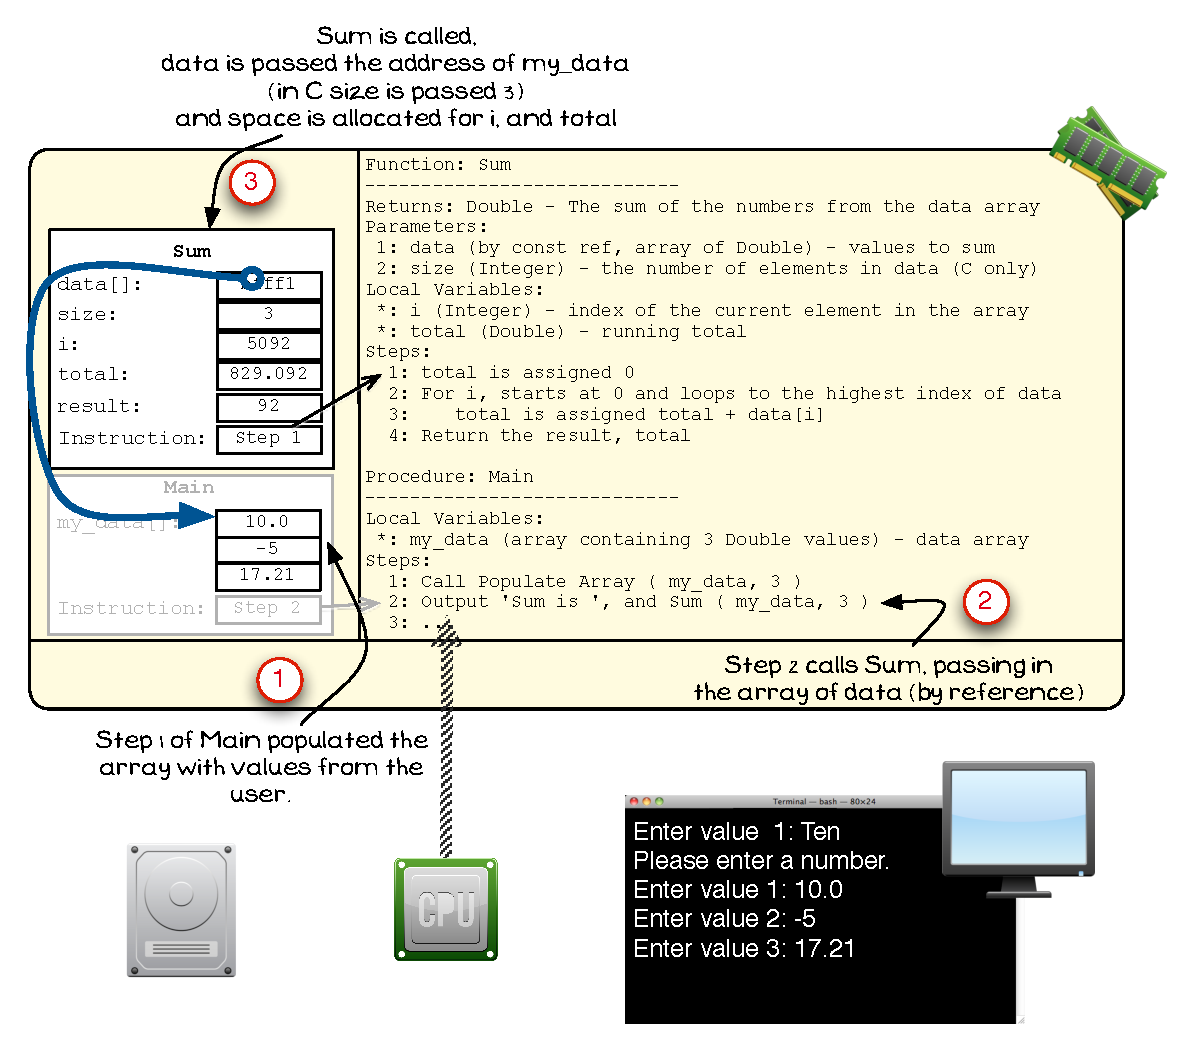
\includegraphics[width=\textwidth]{./topics/arrays/images/Sum1} 
   \caption{\texttt{Sum} is called, and it is passed the array to get its values from}
   \label{fig:sum-array-vis-1}
\end{figure}

\mynote{
\begin{itemize}
  \item In \fref{fig:sum-array-vis-1} the indicated areas show the following:
  \begin{enumerate}
    \item Step 1 of \texttt{Main} has populated the array with values.
    \item Step 2 calls the \texttt{Sum} function, passing in the \texttt{my\_data} array.
    \item When sum starts it is allocated space on the heap. Its \texttt{data} parameter is passed the address of \texttt{my\_data}. In C the \texttt{size} parameter will be passed the value 3, this isn't needed in Pascal as the language takes care of these details for you. Space is also allocated for the local variables \texttt{i} and \texttt{total}.
  \end{enumerate}
  \medskip
  \item Passing \texttt{my\_data} by reference means that sum gets a reference that \emph{points} to the start of the array.
  \item \texttt{Sum} is responsible for calculating the sum value of the values in the array.
  
\end{itemize}
}
% subsubsection sum_is_called_and_passed_the_values_in_my_data (end)

\clearpage
\subsubsection{\texttt{total} is initialised to 0} % (fold)
\label{ssub:total_is_initialised_to_0}

The first action in \texttt{Sum} is to set the value of \texttt{total} to 0. \texttt{total} will be used to store the running total of the array, and it must start at 0. Remember that the space on the stack was used before, and therefore these variables get seemingly random values initially. It is important to remember to always initialise the variables you are using.

\begin{figure}[htbp]
   \centering
   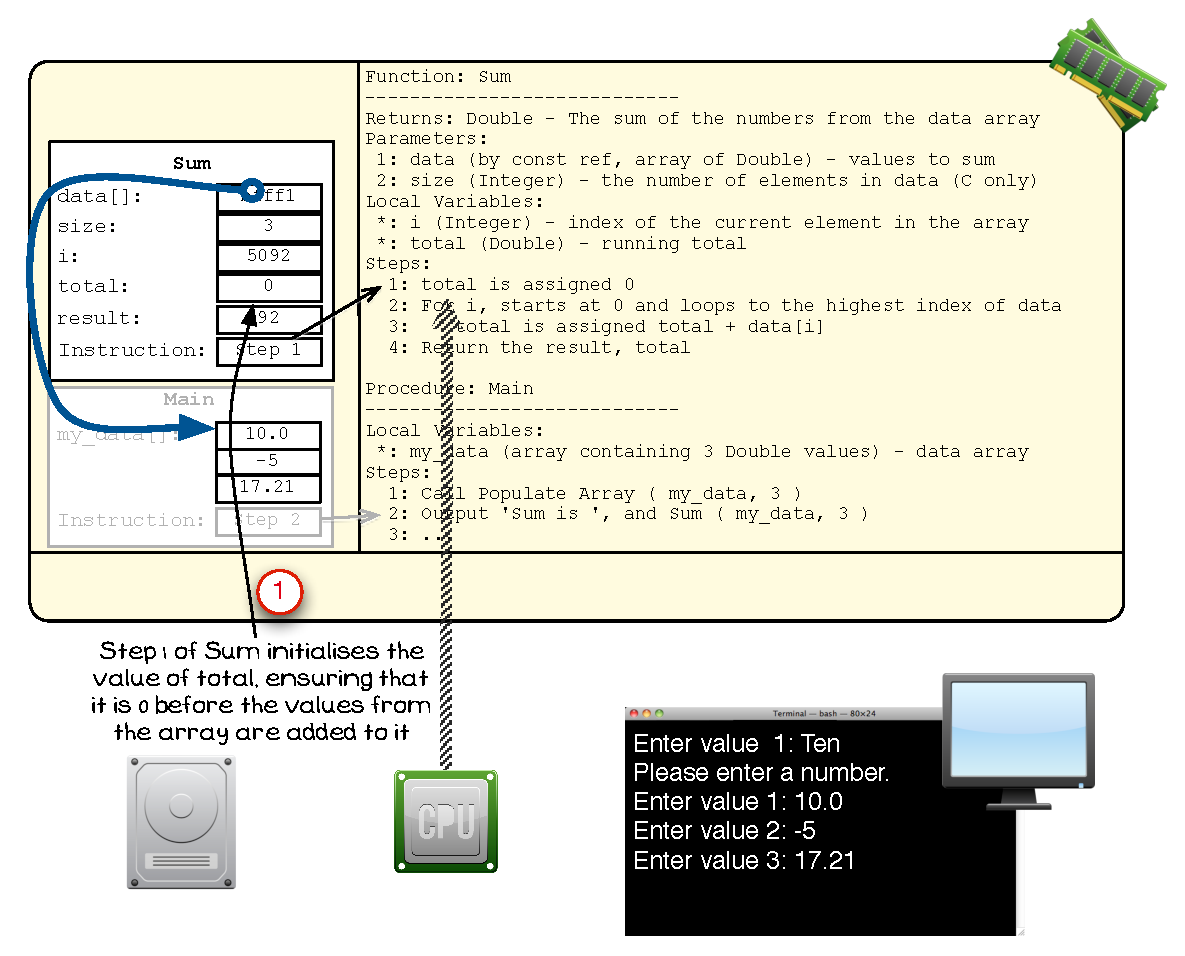
\includegraphics[width=\textwidth]{./topics/arrays/images/Sum2} 
   \caption{\texttt{Total} is initialised, having its value set to 0}
   \label{fig:sum-array-vis-2}
\end{figure}

\mynote{
\begin{itemize}
  \item In \fref{fig:sum-array-vis-2} the indicated areas show the following:
  \begin{enumerate}
    \item The \texttt{total} variable is assigned the value 0.
  \end{enumerate}
  \medskip
  \item Local variables do not get a default value when the Function or Procedure starts. You need to make sure you initialise these to appropriate values before you use them.
  \item \texttt{total} will keep a running total of the elements in the array, it must start at the value 0.
\end{itemize}
}

% subsubsection total_is_initialised_to_0 (end)

\clearpage
\subsubsection{For loop initialises \texttt{i}} % (fold)
\label{ssub:for_loop_initialises_i}

Step 2 of \texttt{Sum} starts the for loop that will iterate over the elements of the \texttt{data} array. The for loop's control variable, \texttt{i}, is set to the first index of the array and the condition checks if the loop's body should run. As \texttt{i} is in the range \texttt{0..2}, it is less than 3, control will jump into the loop's body making step 3 the next instruction.

\begin{figure}[htbp]
   \centering
   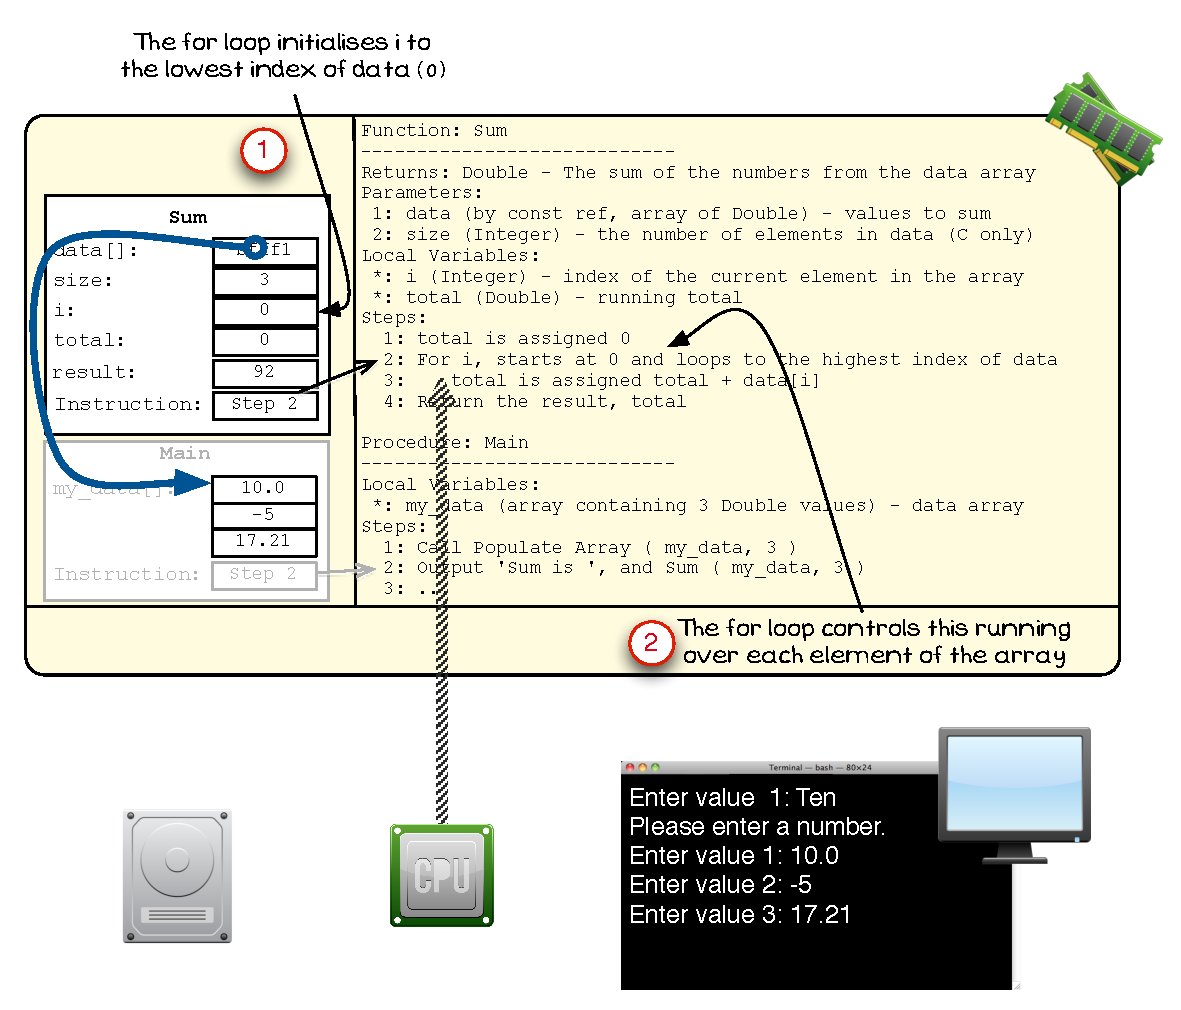
\includegraphics[width=\textwidth]{./topics/arrays/images/Sum3} 
   \caption{\texttt{i} is initialised by the for loop, and control jumps to the loop's body}
   \label{fig:sum-array-vis-3}
\end{figure}

\mynote{
\begin{itemize}
  \item In \fref{fig:sum-array-vis-3} the indicated areas show the following:
  \begin{enumerate}
    \item The for loop initialises its control variable \texttt{i}, assigning it the value 0.
    \item The condition of the loop is checked to see if the body should execute. As \texttt{i} is still in the range \texttt{0..2}, it is less than 3, the loop's body will execute.
  \end{enumerate}
  \medskip
  \item The first action of a for loop is always to initialise its control variable. After this it checks if the body of the loop should run.
\end{itemize}
}

% subsubsection for_loop_initialises_i (end)

\clearpage
\subsubsection{\texttt{total} is increased by the value in \texttt{data[0]}} % (fold)
\label{ssub:total_is_incremented_by_the_value_in_data[0]}

The body of the for loop reads the \emph{current} value from the \texttt{data} array, \texttt{data[i]}. As \texttt{i} is currently 0 this reads the first element of the array. This reads the value 10.0, which is added to the current \texttt{total}, 0. The resulting value is then stored back into the \texttt{total} variable, giving it the value 10.0, calculated from the expression \texttt{total + data[0]}, which is \texttt{0 + 10.0}.

\begin{figure}[htbp]
   \centering
   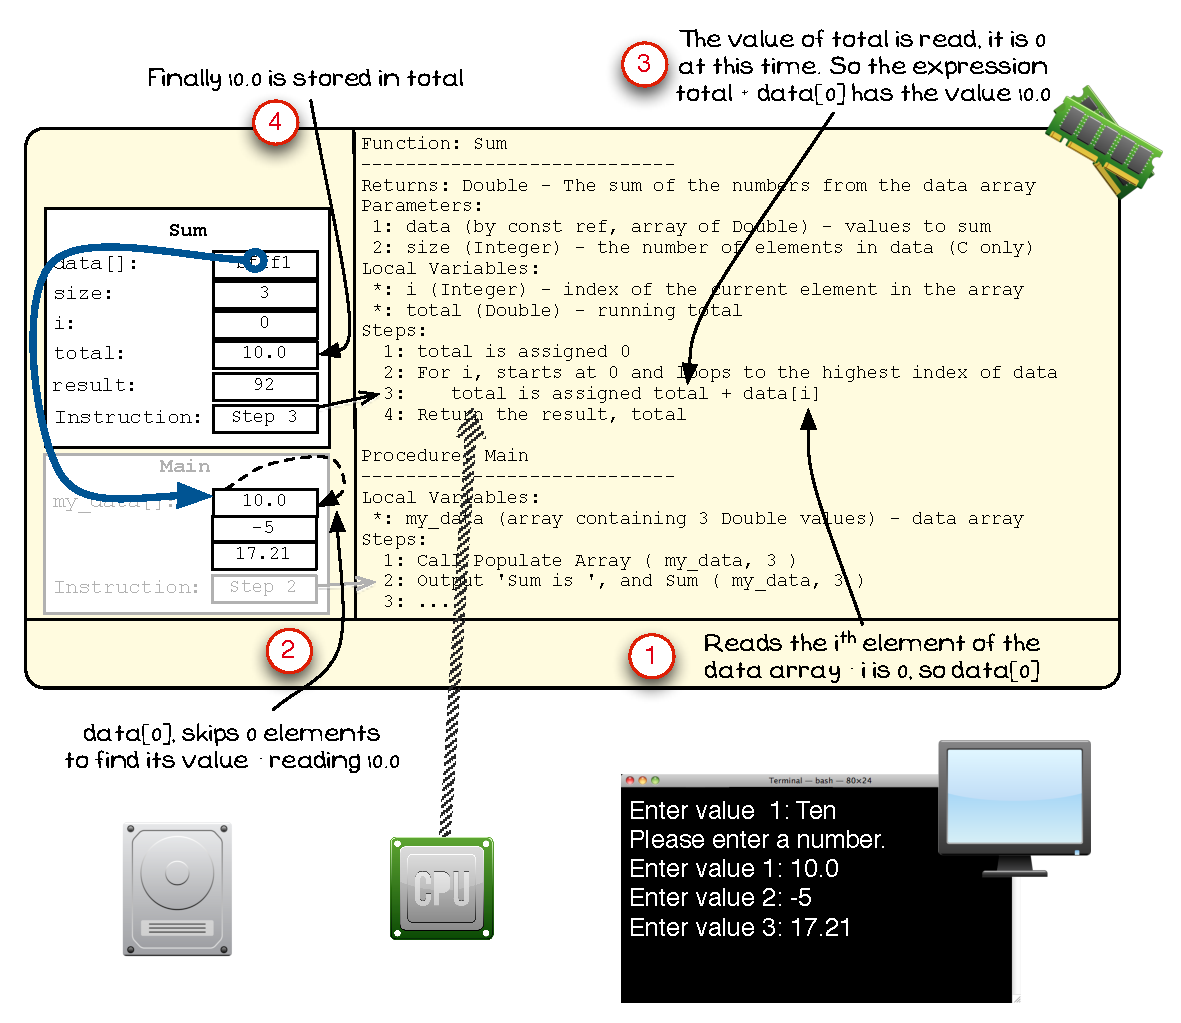
\includegraphics[width=\textwidth]{./topics/arrays/images/Sum4} 
   \caption{Total is increased by the value in \texttt{data[0]}}
   \label{fig:sum-array-vis-4}
\end{figure}

\mynote{
\begin{itemize}
  \item In \fref{fig:sum-array-vis-4} the indicated areas show the following:
  \begin{enumerate}
    \item The value of \texttt{data[i]} must be read in this expression. At this point \texttt{i} is 0, so \texttt{data[0]} must be read.
    \item \texttt{data[0]} is found in the array referred to by \texttt{data}, after skipping \texttt{0} elements. This reads the value of the first array element.
    \item The expression evaluates \texttt{total\footnote{Remember that at this point \texttt{total} has not been changed, so it has the value \texttt{0.0} as shown in \fref{fig:sum-array-vis-3}.} + data[i]}, giving \texttt{total + data[0]}, which is \texttt{0 + 10.0}, with the final value being \texttt{10.0}.
    \item The value 10.0, calculated above, is then stored in \texttt{total}.
  \end{enumerate}
  \medskip
  \item The body of the for loop provides the instructions that are run for each element of the array.
\end{itemize}
}

% subsubsection total_is_incremented_by_the_value_in_data[0] (end)

\clearpage
\subsubsection{For loop increases the value of i and runs the loop body a second time} % (fold)
\label{ssub:for_loop_increases_the_value_of_i_and_runs_the_loop_body_a_second_time}

At the end of the for loop it increments the value of its control variable, assigning \texttt{i} the value 1, and then jumps back to check its condition. As \texttt{i} is still in the range 0..2 the loop body will be run again, making step 3 the next action. 

\begin{figure}[htbp]
   \centering
   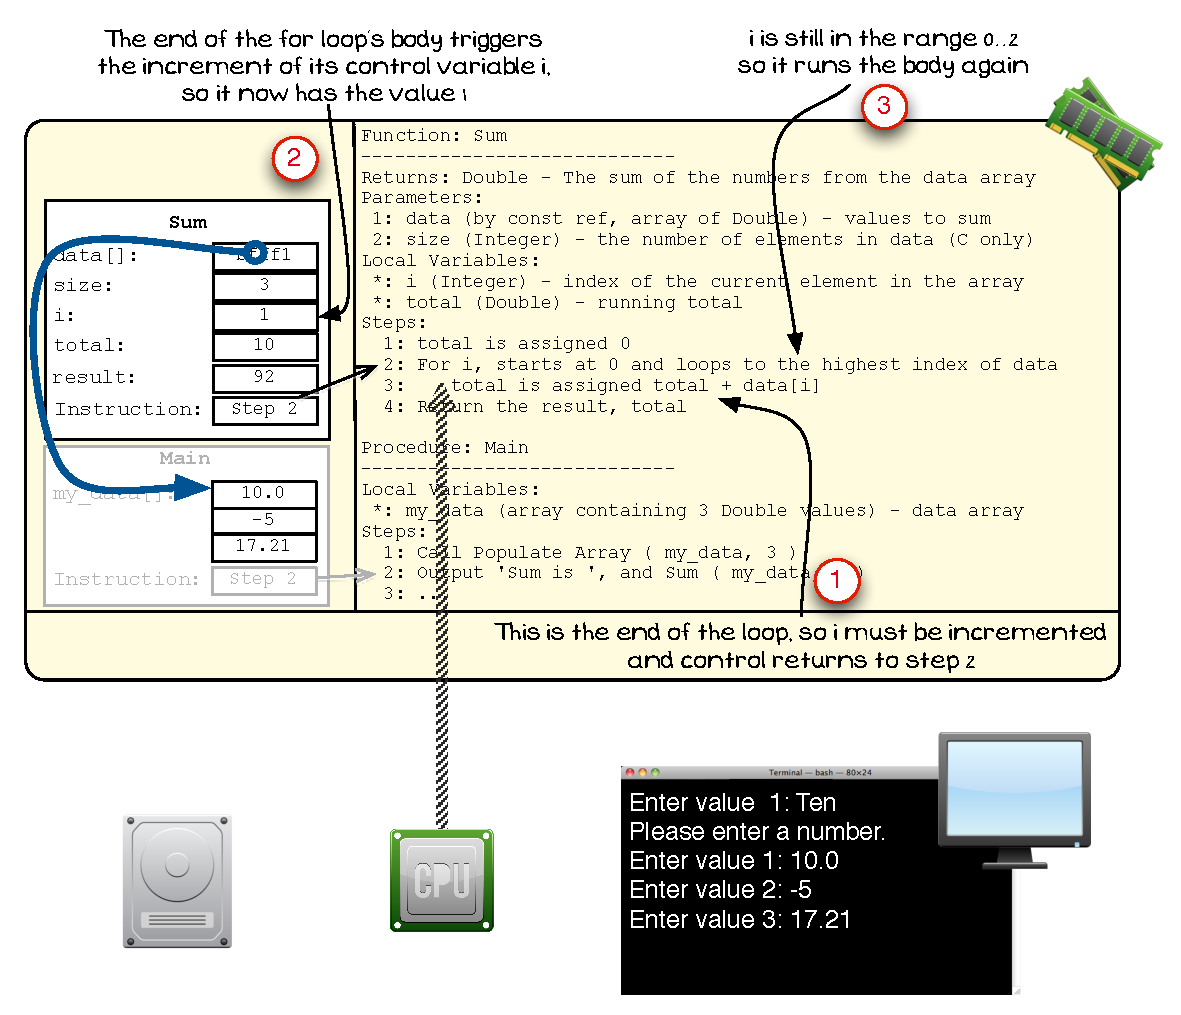
\includegraphics[width=0.95\textwidth]{./topics/arrays/images/Sum5} 
   \caption{At the end of the loop body \texttt{i} is incremented, and control jumps back to check the condition}
   \label{fig:sum-array-vis-5}
\end{figure}

\mynote{
\begin{itemize}
  \item In \fref{fig:sum-array-vis-5} the indicated areas show the following:
  \begin{enumerate}
    \item The end of the loop has been reached. The for loop increments its control variable, and jumps back to check its condition.
    \item In this case \texttt{i} is the control variable, so its value is increased to 1.
    \item The condition of the loop is checked to see if the body should execute. As \texttt{i} is still in the range \texttt{0..2} (it is less than 3) the loop's body will execute, making step 3 the next action.
  \end{enumerate}
  \medskip
  \item The end of each for loop always performs these steps. Increasing the value of its control variable, and jumping back to check its condition.
\end{itemize}
}

\csection{Remember C can do more than just counting in the for loop, though this is its main use.}


% subsubsection for_loop_increases_the_value_of_i_and_runs_the_loop_body_a_second_time (end)

\clearpage
\subsubsection{The value of \texttt{total} is increased by the value in \texttt{data[1]}} % (fold)
\label{ssub:the_value_of_total_is_increased_by_the_value_in_data[1]}

The body of the for loop reads the \emph{current} value from the \texttt{data} array, \texttt{data[i]}. Now \texttt{i} has the value 1 it reads the second element of the array. This reads the value -5, which is added to the current \texttt{total}, 10.0. The resulting value is then stored back into the \texttt{total} variable, giving it the value 5.0, calculated from the expression \texttt{total + data[1]}, which is \texttt{10.0 + -5.0}.

\begin{figure}[htbp]
   \centering
   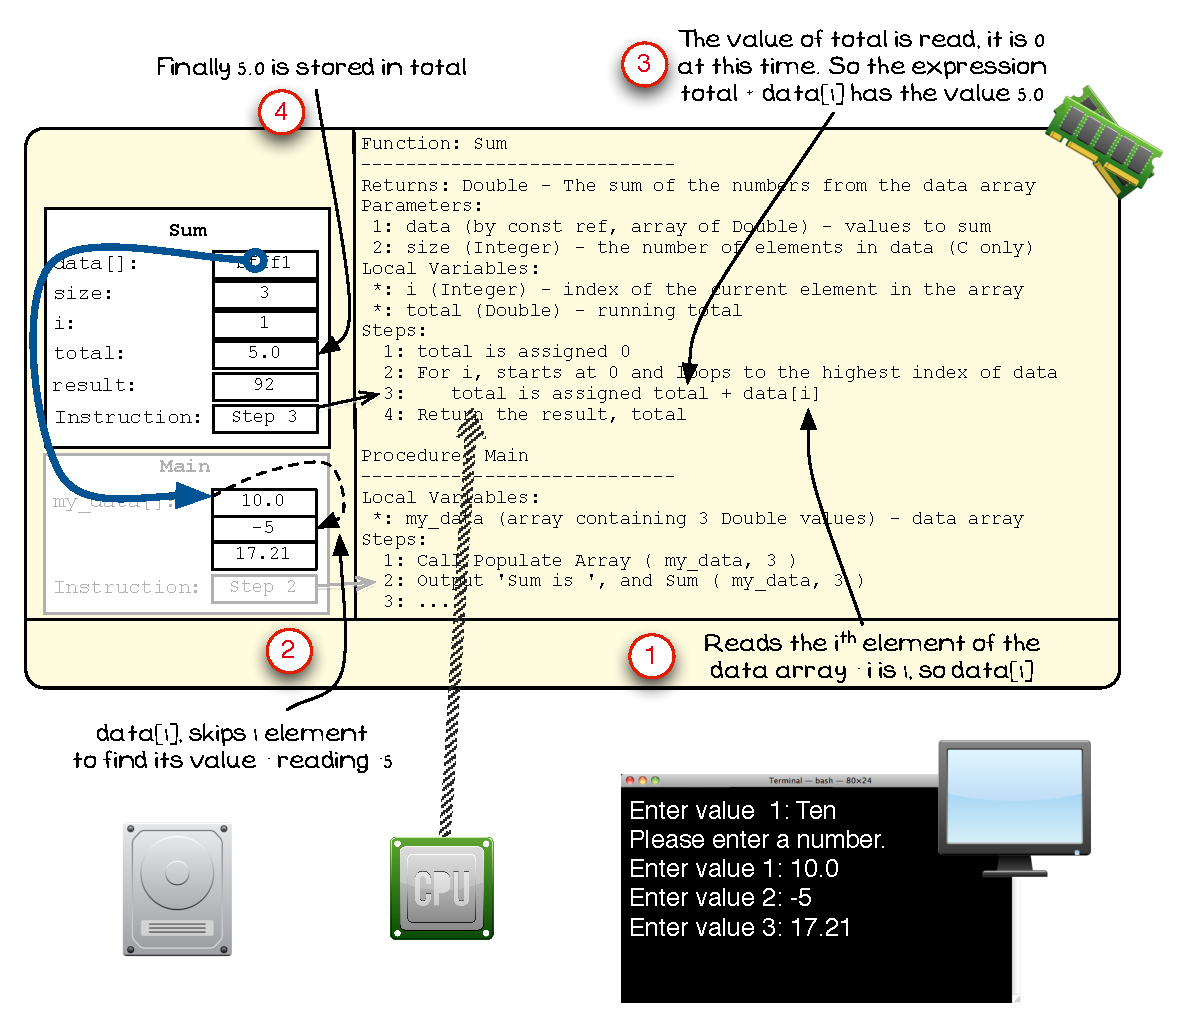
\includegraphics[width=\textwidth]{./topics/arrays/images/Sum6} 
   \caption{Total is increased by the value in \texttt{data[1]}}
   \label{fig:sum-array-vis-6}
\end{figure}

\mynote{
\begin{itemize}
  \item In \fref{fig:sum-array-vis-6} the indicated areas show the following:
  \begin{enumerate}
    \item The value of \texttt{data[i]} must be read in this expression. At this point \texttt{i} is 1, so \texttt{data[1]} must be read.
    \item \texttt{data[1]} is found in the array referred to by \texttt{data}, after skipping \texttt{1} element. This reads the value of the second array element.
    \item The expression evaluates \texttt{total\footnote{As before, \texttt{total} has not been changed at this point, so it has the value \texttt{10.0} as shown in \fref{fig:sum-array-vis-5}.} + data[i]}, giving \texttt{total + data[1]}, which is \texttt{10.0 + -5.0}, with the final value being \texttt{5.0}.
    \item The value 5.0, calculated above, is then stored in \texttt{total}.
  \end{enumerate}
  \medskip
  \item Notice that this is performing the same task, just using the next element from the array.
\end{itemize}
}

% subsubsection the_value_of_total_is_increased_by_the_value_in_data[1] (end)

\clearpage
\subsubsection{For loop increases the value of i and runs the loop body a third time} % (fold)
\label{ssub:for_loop_increases_the_value_of_i_and_runs_the_loop_body_a_third_time}

The end of the for loop has been reached again, so it increments the value of its control variable, assigning \texttt{i} the value 2, and then jumps back to check its condition. As \texttt{i} is still in the range 0..2 the loop body will run a third time, making step 3 the next action. 

\begin{figure}[htbp]
   \centering
   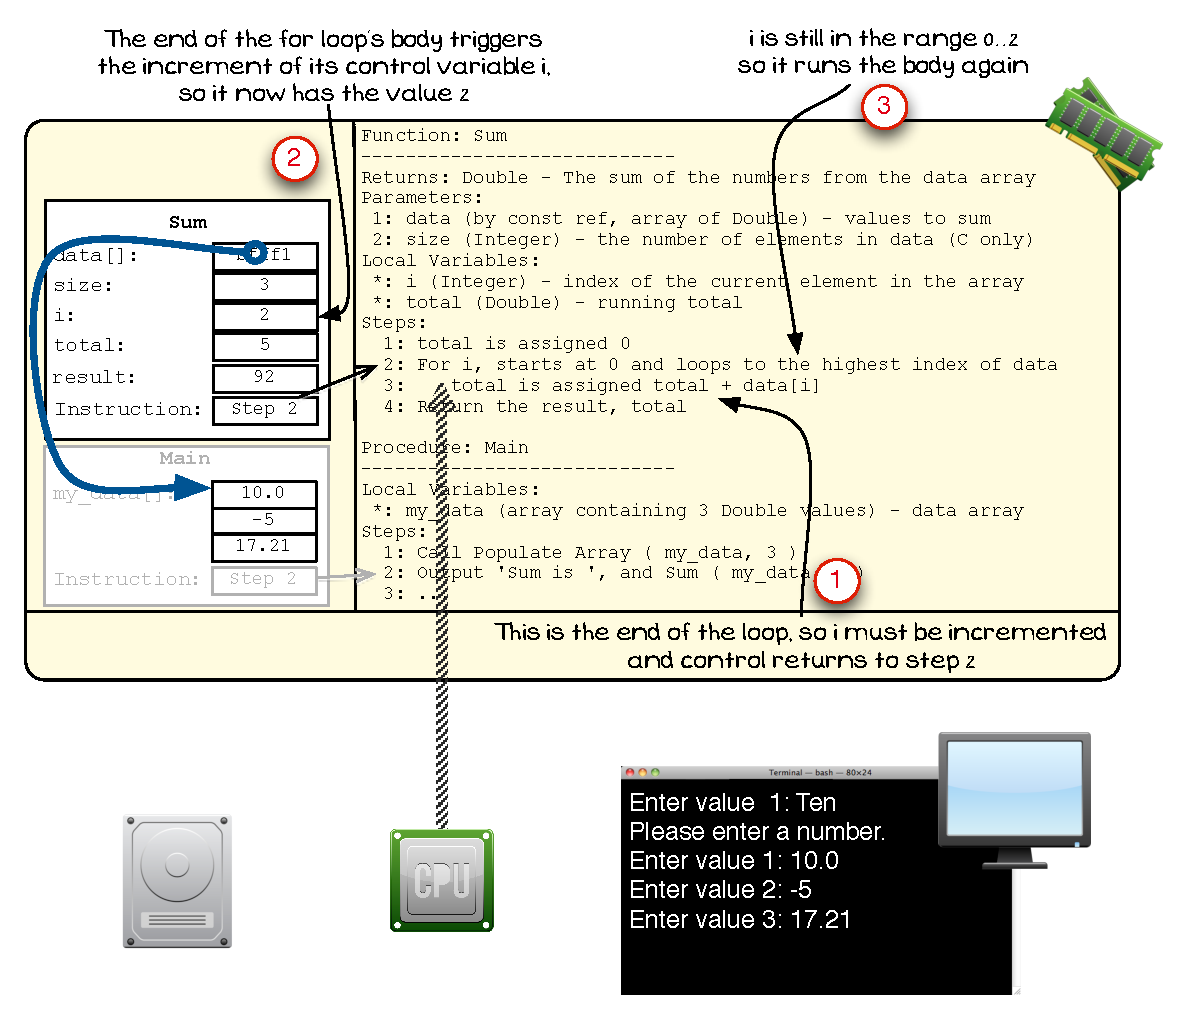
\includegraphics[width=0.95\textwidth]{./topics/arrays/images/Sum7} 
   \caption{At the end of the loop body \texttt{i} is incremented, and control jumps back to check the condition}
   \label{fig:sum-array-vis-7}
\end{figure}

\mynote{
\begin{itemize}
  \item In \fref{fig:sum-array-vis-7} the indicated areas show the following:
  \begin{enumerate}
    \item The end of the loop has been reached. The for loop increments its control variable, and jumps back to check its condition.
    \item In this case \texttt{i} is the control variable, so its value is increased to 2.
    \item The condition of the loop is checked to see if the body should execute. As \texttt{i} is still in the range \texttt{0..2} (it is less than 3) the loop's body will execute, making step 3 the next action.
  \end{enumerate}
  \medskip
  \item The end of each for loop always performs these steps. Increasing the value of its control variable, and jumping back to check its condition.
\end{itemize}
}

% subsubsection for_loop_increases_the_value_of_i_and_runs_the_loop_body_a_third_time (end)

\clearpage
\subsubsection{The value of \texttt{total} is increased by the value in \texttt{data[2]}} % (fold)
\label{ssub:the_value_of_total_is_increased_by_the_value_in_data[2]}

The body of the for loop reads the \emph{current} value from the \texttt{data} array, \texttt{data[i]}. Now \texttt{i} has the value 2 it reads the second element of the array. This reads the value 17.21, which is added to the current \texttt{total}, 5.0. The resulting value is then stored back into the \texttt{total} variable, giving it the value 22.21, calculated from the expression \texttt{total + data[2]}, which is \texttt{5.0 + 17.21}.

\begin{figure}[htbp]
   \centering
   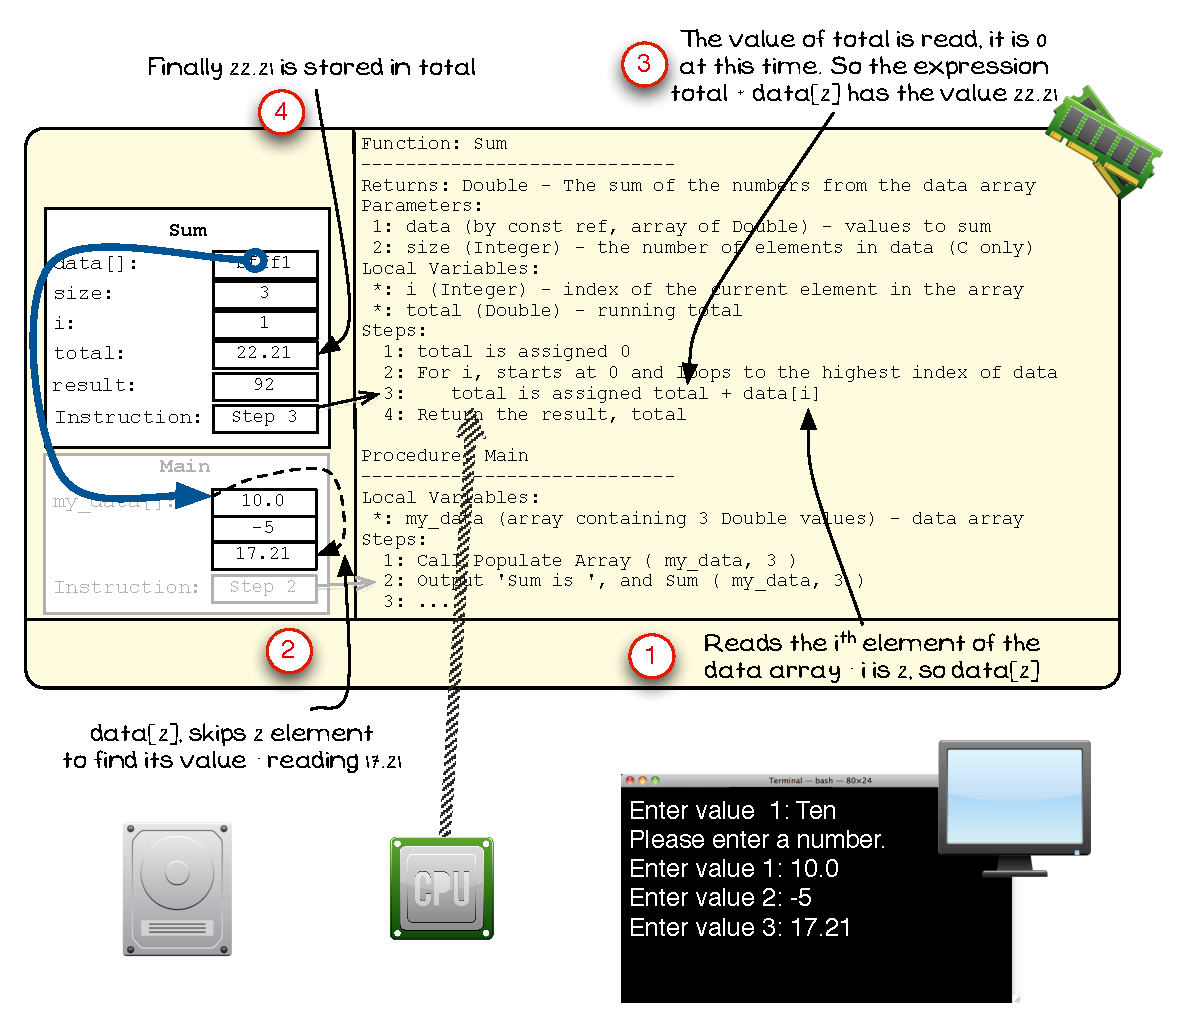
\includegraphics[width=\textwidth]{./topics/arrays/images/Sum8} 
   \caption{Total is increased by the value in \texttt{data[1]}}
   \label{fig:sum-array-vis-8}
\end{figure}

\mynote{
\begin{itemize}
  \item In \fref{fig:sum-array-vis-8} the indicated areas show the following:
  \begin{enumerate}
    \item The value of \texttt{data[i]} must be read in this expression. At this point \texttt{i} is 2, so \texttt{data[2]} must be read.
    \item \texttt{data[2]} is found in the array referred to by \texttt{data}, after skipping \texttt{2} elements. This reads the value of the third array element.
    \item The expression evaluates \texttt{total\footnote{As before, \texttt{total} has not been changed at this point, so it has the value \texttt{5.0} as shown in \fref{fig:sum-array-vis-7}.} + data[i]}, giving \texttt{total + data[2]}, which is \texttt{5.0 + 17.21}, with the final value being \texttt{22.21}.
    \item The value 5.0, calculated above, is then stored in \texttt{total}.
  \end{enumerate}
  \medskip
  \item Notice that this is performing the same task, just using the next element from the array.
\end{itemize}
}

% subsubsection the_value_of_total_is_increased_by_the_value_in_data[2] (end)

\clearpage
\subsubsection{For loop increases the value of \texttt{i}, and this time the loop finishes} % (fold)
\label{ssub:for_loop_increases_the_value_of_i_and_this_time_the_loop_finishes}

The end of the for loop has been reached again, so it increments the value of its control variable, assigning \texttt{i} the value 3, and then jumps back to check its condition. This time \texttt{i} is no longer in the range 0..2 (it is not less than 3), so the loop body will now be skipped, making step 4 the next action. 

\begin{figure}[htbp]
   \centering
   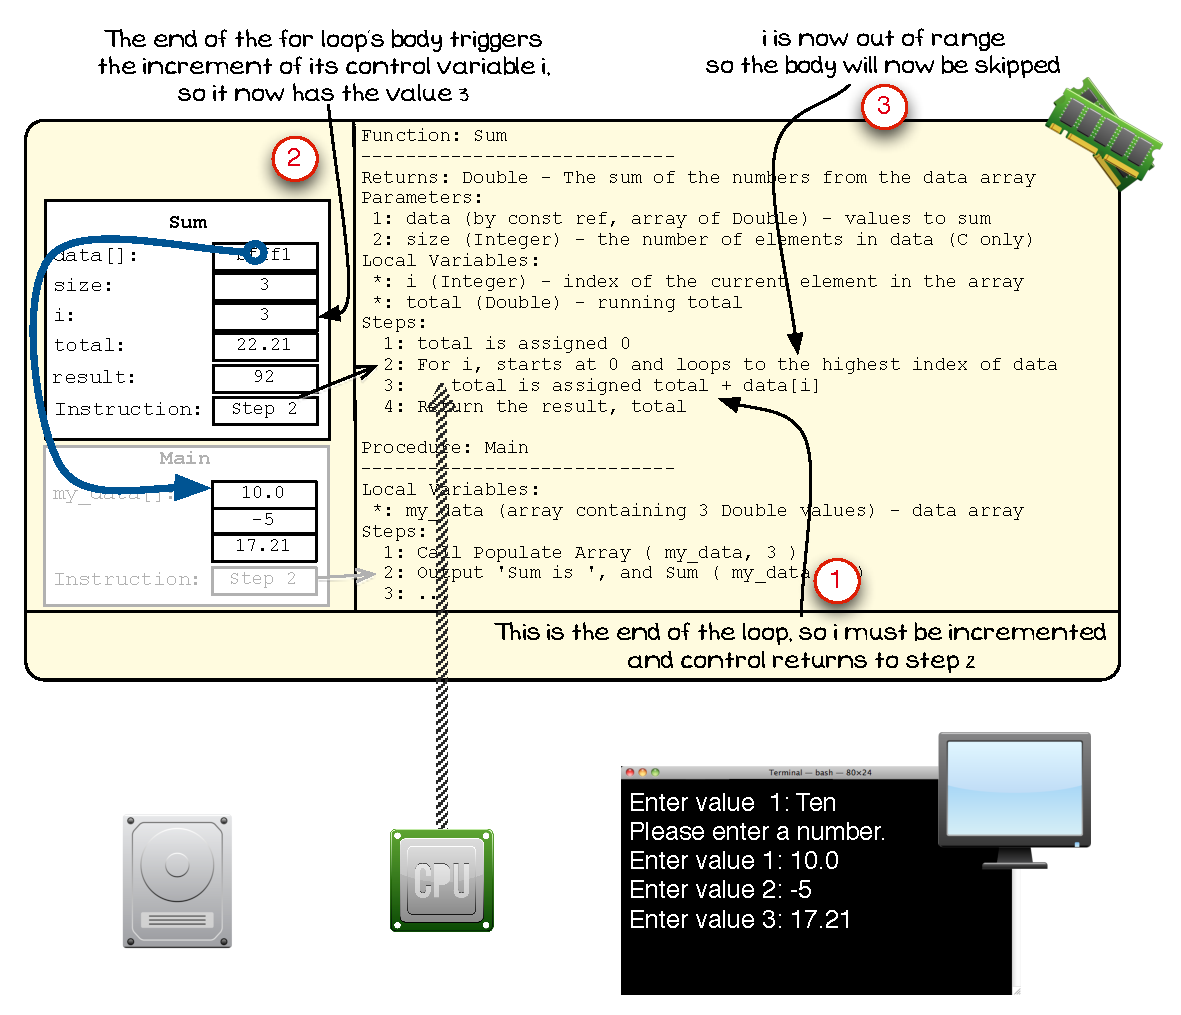
\includegraphics[width=0.95\textwidth]{./topics/arrays/images/Sum9} 
   \caption{At the end of the loop body \texttt{i} is incremented, and control jumps back to check the condition}
   \label{fig:sum-array-vis-9}
\end{figure}

\mynote{
\begin{itemize}
  \item In \fref{fig:sum-array-vis-9} the indicated areas show the following:
  \begin{enumerate}
    \item The end of the loop has been reached. The for loop increments its control variable, and jumps back to check its condition.
    \item In this case \texttt{i} is the control variable, so its value is increased to 3.
    \item The condition of the loop is checked to see if the body should execute. \texttt{i} is no longer in the range \texttt{0..2} (it is not less than 3), so the loop's body will be skipped, making step 4 the next action.
  \end{enumerate}
  \medskip
  \item The for works just like a while loop, checking its condition each loop and skipping the body when the condition is not met (when it is false).
\end{itemize}
}

% subsubsection for_loop_increases_the_value_of_i_and_this_time_the_loop_finishes (end)

\clearpage
\subsubsection{\texttt{Sum} function returns the \texttt{total} to the expression in \texttt{Main}} % (fold)
\label{ssub:sum_function_returns_the_total_to_the_expression_in_main}

The end of the for loop has been reached again, so it increments the value of its control variable, assigning \texttt{i} the value 3, and then jumps back to check its condition. This time \texttt{i} is no longer in the range 0..2 (it is not less than 3), so the loop body will now be skipped, making step 4 the next action. 

\begin{figure}[htbp]
   \centering
   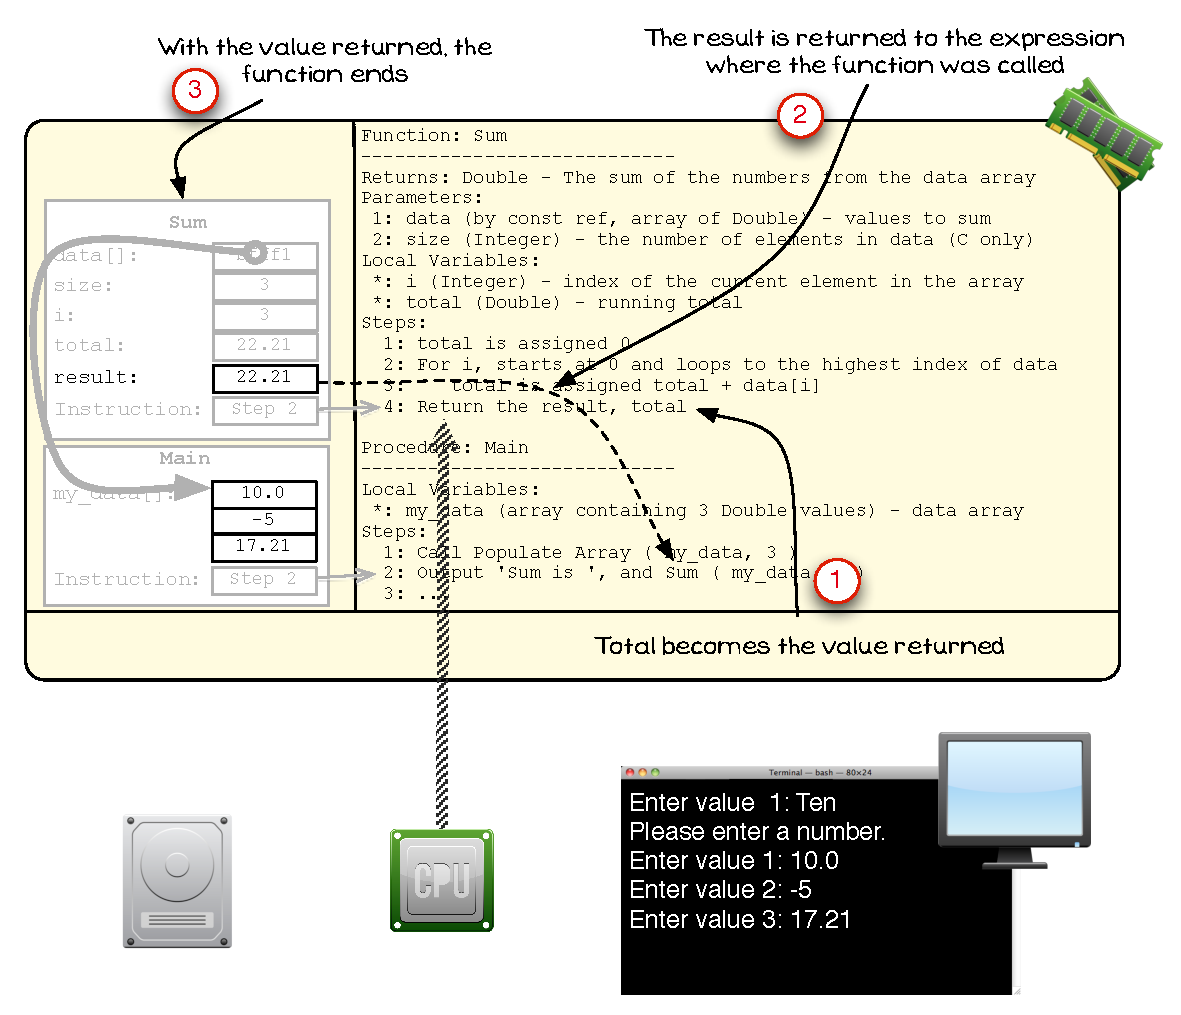
\includegraphics[width=0.95\textwidth]{./topics/arrays/images/Sum10} 
   \caption{Step 4 indicates that the value in \texttt{total} is returned to \texttt{Main}}
   \label{fig:sum-array-vis-10}
\end{figure}

\mynote{
\begin{itemize}
  \item In \fref{fig:sum-array-vis-10} the indicated areas show the following:
  \begin{enumerate}
    \item Step 4 indicates that the value in the \texttt{total} variable should be returned to the caller.
    \item The result returned by the \texttt{Sum} function is used in the expression in \texttt{Main}.
    \item As this is the end of the function its space on the stack is released, allowing control to return to \texttt{Main}.
  \end{enumerate}
  \medskip
  \item The for works just like a while loop, checking its condition each loop and skipping the body when the condition is not met (when it is false).
\end{itemize}
}

% subsubsection sum_function_returns_the_total_to_the_expression_in_main (end)

\clearpage
\subsubsection{\texttt{Main} outputs the sum to the Terminal} % (fold)
\label{ssub:main_outputs_the_sum_to_the_terminal}

\texttt{Sum} returns its value to be used in step 2 of \texttt{Main}. This step outputs the value returned to the Terminal. So by the end of Step 2 in \texttt{Main} the sum has been calculated, and written to the Terminal.

\begin{figure}[htbp]
   \centering
   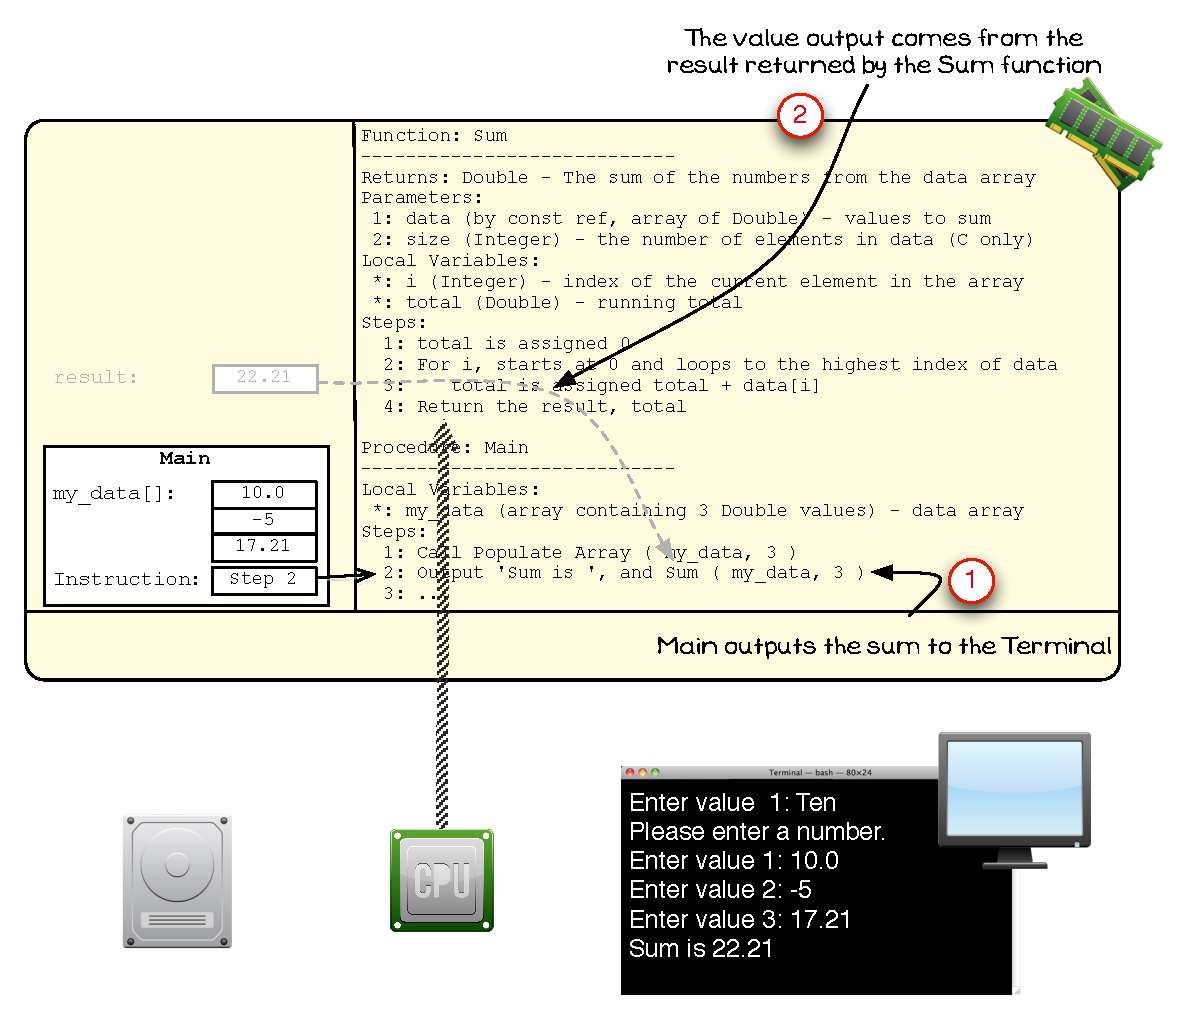
\includegraphics[width=0.95\textwidth]{./topics/arrays/images/Sum11} 
   \caption{Step 4 indicates that the value in \texttt{total} is returned to \texttt{Main}}
   \label{fig:sum-array-vis-11}
\end{figure}

\mynote{
\begin{itemize}
  \item In \fref{fig:sum-array-vis-11} the indicated areas show the following:
  \begin{enumerate}
    \item Back in \texttt{Main}, the sum is output to the Terminal.
    \item The value that is output is the value returned from the \texttt{Sum} function.
  \end{enumerate}
\end{itemize}
}

% subsubsection main_outputs_the_sum_to_the_terminal (end)

% subsection understanding_sum (end)
